
% Default to the notebook output style

    


% Inherit from the specified cell style.




    
\documentclass{article}

    
    
    \usepackage{graphicx} % Used to insert images
    \usepackage{adjustbox} % Used to constrain images to a maximum size 
    \usepackage{color} % Allow colors to be defined
    \usepackage{enumerate} % Needed for markdown enumerations to work
    \usepackage{geometry} % Used to adjust the document margins
    \usepackage{amsmath} % Equations
    \usepackage{amssymb} % Equations
    \usepackage[mathletters]{ucs} % Extended unicode (utf-8) support
    \usepackage[utf8x]{inputenc} % Allow utf-8 characters in the tex document
    \usepackage{fancyvrb} % verbatim replacement that allows latex
    \usepackage{grffile} % extends the file name processing of package graphics 
                         % to support a larger range 
    % The hyperref package gives us a pdf with properly built
    % internal navigation ('pdf bookmarks' for the table of contents,
    % internal cross-reference links, web links for URLs, etc.)
    \usepackage{hyperref}
    \usepackage{longtable} % longtable support required by pandoc >1.10
    

    
    
    \definecolor{orange}{cmyk}{0,0.4,0.8,0.2}
    \definecolor{darkorange}{rgb}{.71,0.21,0.01}
    \definecolor{darkgreen}{rgb}{.12,.54,.11}
    \definecolor{myteal}{rgb}{.26, .44, .56}
    \definecolor{gray}{gray}{0.45}
    \definecolor{lightgray}{gray}{.95}
    \definecolor{mediumgray}{gray}{.8}
    \definecolor{inputbackground}{rgb}{.95, .95, .85}
    \definecolor{outputbackground}{rgb}{.95, .95, .95}
    \definecolor{traceback}{rgb}{1, .95, .95}
    % ansi colors
    \definecolor{red}{rgb}{.6,0,0}
    \definecolor{green}{rgb}{0,.65,0}
    \definecolor{brown}{rgb}{0.6,0.6,0}
    \definecolor{blue}{rgb}{0,.145,.698}
    \definecolor{purple}{rgb}{.698,.145,.698}
    \definecolor{cyan}{rgb}{0,.698,.698}
    \definecolor{lightgray}{gray}{0.5}
    
    % bright ansi colors
    \definecolor{darkgray}{gray}{0.25}
    \definecolor{lightred}{rgb}{1.0,0.39,0.28}
    \definecolor{lightgreen}{rgb}{0.48,0.99,0.0}
    \definecolor{lightblue}{rgb}{0.53,0.81,0.92}
    \definecolor{lightpurple}{rgb}{0.87,0.63,0.87}
    \definecolor{lightcyan}{rgb}{0.5,1.0,0.83}
    
    % commands and environments needed by pandoc snippets
    % extracted from the output of `pandoc -s`
    \DefineVerbatimEnvironment{Highlighting}{Verbatim}{commandchars=\\\{\}}
    % Add ',fontsize=\small' for more characters per line
    \newenvironment{Shaded}{}{}
    \newcommand{\KeywordTok}[1]{\textcolor[rgb]{0.00,0.44,0.13}{\textbf{{#1}}}}
    \newcommand{\DataTypeTok}[1]{\textcolor[rgb]{0.56,0.13,0.00}{{#1}}}
    \newcommand{\DecValTok}[1]{\textcolor[rgb]{0.25,0.63,0.44}{{#1}}}
    \newcommand{\BaseNTok}[1]{\textcolor[rgb]{0.25,0.63,0.44}{{#1}}}
    \newcommand{\FloatTok}[1]{\textcolor[rgb]{0.25,0.63,0.44}{{#1}}}
    \newcommand{\CharTok}[1]{\textcolor[rgb]{0.25,0.44,0.63}{{#1}}}
    \newcommand{\StringTok}[1]{\textcolor[rgb]{0.25,0.44,0.63}{{#1}}}
    \newcommand{\CommentTok}[1]{\textcolor[rgb]{0.38,0.63,0.69}{\textit{{#1}}}}
    \newcommand{\OtherTok}[1]{\textcolor[rgb]{0.00,0.44,0.13}{{#1}}}
    \newcommand{\AlertTok}[1]{\textcolor[rgb]{1.00,0.00,0.00}{\textbf{{#1}}}}
    \newcommand{\FunctionTok}[1]{\textcolor[rgb]{0.02,0.16,0.49}{{#1}}}
    \newcommand{\RegionMarkerTok}[1]{{#1}}
    \newcommand{\ErrorTok}[1]{\textcolor[rgb]{1.00,0.00,0.00}{\textbf{{#1}}}}
    \newcommand{\NormalTok}[1]{{#1}}
    
    % Define a nice break command that doesn't care if a line doesn't already
    % exist.
    \def\br{\hspace*{\fill} \\* }
    % Math Jax compatability definitions
    \def\gt{>}
    \def\lt{<}
    % Document parameters
    \title{AG}
    
    
    

    % Pygments definitions
    
\makeatletter
\def\PY@reset{\let\PY@it=\relax \let\PY@bf=\relax%
    \let\PY@ul=\relax \let\PY@tc=\relax%
    \let\PY@bc=\relax \let\PY@ff=\relax}
\def\PY@tok#1{\csname PY@tok@#1\endcsname}
\def\PY@toks#1+{\ifx\relax#1\empty\else%
    \PY@tok{#1}\expandafter\PY@toks\fi}
\def\PY@do#1{\PY@bc{\PY@tc{\PY@ul{%
    \PY@it{\PY@bf{\PY@ff{#1}}}}}}}
\def\PY#1#2{\PY@reset\PY@toks#1+\relax+\PY@do{#2}}

\expandafter\def\csname PY@tok@gd\endcsname{\def\PY@tc##1{\textcolor[rgb]{0.63,0.00,0.00}{##1}}}
\expandafter\def\csname PY@tok@gu\endcsname{\let\PY@bf=\textbf\def\PY@tc##1{\textcolor[rgb]{0.50,0.00,0.50}{##1}}}
\expandafter\def\csname PY@tok@gt\endcsname{\def\PY@tc##1{\textcolor[rgb]{0.00,0.27,0.87}{##1}}}
\expandafter\def\csname PY@tok@gs\endcsname{\let\PY@bf=\textbf}
\expandafter\def\csname PY@tok@gr\endcsname{\def\PY@tc##1{\textcolor[rgb]{1.00,0.00,0.00}{##1}}}
\expandafter\def\csname PY@tok@cm\endcsname{\let\PY@it=\textit\def\PY@tc##1{\textcolor[rgb]{0.25,0.50,0.50}{##1}}}
\expandafter\def\csname PY@tok@vg\endcsname{\def\PY@tc##1{\textcolor[rgb]{0.10,0.09,0.49}{##1}}}
\expandafter\def\csname PY@tok@m\endcsname{\def\PY@tc##1{\textcolor[rgb]{0.40,0.40,0.40}{##1}}}
\expandafter\def\csname PY@tok@mh\endcsname{\def\PY@tc##1{\textcolor[rgb]{0.40,0.40,0.40}{##1}}}
\expandafter\def\csname PY@tok@go\endcsname{\def\PY@tc##1{\textcolor[rgb]{0.53,0.53,0.53}{##1}}}
\expandafter\def\csname PY@tok@ge\endcsname{\let\PY@it=\textit}
\expandafter\def\csname PY@tok@vc\endcsname{\def\PY@tc##1{\textcolor[rgb]{0.10,0.09,0.49}{##1}}}
\expandafter\def\csname PY@tok@il\endcsname{\def\PY@tc##1{\textcolor[rgb]{0.40,0.40,0.40}{##1}}}
\expandafter\def\csname PY@tok@cs\endcsname{\let\PY@it=\textit\def\PY@tc##1{\textcolor[rgb]{0.25,0.50,0.50}{##1}}}
\expandafter\def\csname PY@tok@cp\endcsname{\def\PY@tc##1{\textcolor[rgb]{0.74,0.48,0.00}{##1}}}
\expandafter\def\csname PY@tok@gi\endcsname{\def\PY@tc##1{\textcolor[rgb]{0.00,0.63,0.00}{##1}}}
\expandafter\def\csname PY@tok@gh\endcsname{\let\PY@bf=\textbf\def\PY@tc##1{\textcolor[rgb]{0.00,0.00,0.50}{##1}}}
\expandafter\def\csname PY@tok@ni\endcsname{\let\PY@bf=\textbf\def\PY@tc##1{\textcolor[rgb]{0.60,0.60,0.60}{##1}}}
\expandafter\def\csname PY@tok@nl\endcsname{\def\PY@tc##1{\textcolor[rgb]{0.63,0.63,0.00}{##1}}}
\expandafter\def\csname PY@tok@nn\endcsname{\let\PY@bf=\textbf\def\PY@tc##1{\textcolor[rgb]{0.00,0.00,1.00}{##1}}}
\expandafter\def\csname PY@tok@no\endcsname{\def\PY@tc##1{\textcolor[rgb]{0.53,0.00,0.00}{##1}}}
\expandafter\def\csname PY@tok@na\endcsname{\def\PY@tc##1{\textcolor[rgb]{0.49,0.56,0.16}{##1}}}
\expandafter\def\csname PY@tok@nb\endcsname{\def\PY@tc##1{\textcolor[rgb]{0.00,0.50,0.00}{##1}}}
\expandafter\def\csname PY@tok@nc\endcsname{\let\PY@bf=\textbf\def\PY@tc##1{\textcolor[rgb]{0.00,0.00,1.00}{##1}}}
\expandafter\def\csname PY@tok@nd\endcsname{\def\PY@tc##1{\textcolor[rgb]{0.67,0.13,1.00}{##1}}}
\expandafter\def\csname PY@tok@ne\endcsname{\let\PY@bf=\textbf\def\PY@tc##1{\textcolor[rgb]{0.82,0.25,0.23}{##1}}}
\expandafter\def\csname PY@tok@nf\endcsname{\def\PY@tc##1{\textcolor[rgb]{0.00,0.00,1.00}{##1}}}
\expandafter\def\csname PY@tok@si\endcsname{\let\PY@bf=\textbf\def\PY@tc##1{\textcolor[rgb]{0.73,0.40,0.53}{##1}}}
\expandafter\def\csname PY@tok@s2\endcsname{\def\PY@tc##1{\textcolor[rgb]{0.73,0.13,0.13}{##1}}}
\expandafter\def\csname PY@tok@vi\endcsname{\def\PY@tc##1{\textcolor[rgb]{0.10,0.09,0.49}{##1}}}
\expandafter\def\csname PY@tok@nt\endcsname{\let\PY@bf=\textbf\def\PY@tc##1{\textcolor[rgb]{0.00,0.50,0.00}{##1}}}
\expandafter\def\csname PY@tok@nv\endcsname{\def\PY@tc##1{\textcolor[rgb]{0.10,0.09,0.49}{##1}}}
\expandafter\def\csname PY@tok@s1\endcsname{\def\PY@tc##1{\textcolor[rgb]{0.73,0.13,0.13}{##1}}}
\expandafter\def\csname PY@tok@sh\endcsname{\def\PY@tc##1{\textcolor[rgb]{0.73,0.13,0.13}{##1}}}
\expandafter\def\csname PY@tok@sc\endcsname{\def\PY@tc##1{\textcolor[rgb]{0.73,0.13,0.13}{##1}}}
\expandafter\def\csname PY@tok@sx\endcsname{\def\PY@tc##1{\textcolor[rgb]{0.00,0.50,0.00}{##1}}}
\expandafter\def\csname PY@tok@bp\endcsname{\def\PY@tc##1{\textcolor[rgb]{0.00,0.50,0.00}{##1}}}
\expandafter\def\csname PY@tok@c1\endcsname{\let\PY@it=\textit\def\PY@tc##1{\textcolor[rgb]{0.25,0.50,0.50}{##1}}}
\expandafter\def\csname PY@tok@kc\endcsname{\let\PY@bf=\textbf\def\PY@tc##1{\textcolor[rgb]{0.00,0.50,0.00}{##1}}}
\expandafter\def\csname PY@tok@c\endcsname{\let\PY@it=\textit\def\PY@tc##1{\textcolor[rgb]{0.25,0.50,0.50}{##1}}}
\expandafter\def\csname PY@tok@mf\endcsname{\def\PY@tc##1{\textcolor[rgb]{0.40,0.40,0.40}{##1}}}
\expandafter\def\csname PY@tok@err\endcsname{\def\PY@bc##1{\setlength{\fboxsep}{0pt}\fcolorbox[rgb]{1.00,0.00,0.00}{1,1,1}{\strut ##1}}}
\expandafter\def\csname PY@tok@kd\endcsname{\let\PY@bf=\textbf\def\PY@tc##1{\textcolor[rgb]{0.00,0.50,0.00}{##1}}}
\expandafter\def\csname PY@tok@ss\endcsname{\def\PY@tc##1{\textcolor[rgb]{0.10,0.09,0.49}{##1}}}
\expandafter\def\csname PY@tok@sr\endcsname{\def\PY@tc##1{\textcolor[rgb]{0.73,0.40,0.53}{##1}}}
\expandafter\def\csname PY@tok@mo\endcsname{\def\PY@tc##1{\textcolor[rgb]{0.40,0.40,0.40}{##1}}}
\expandafter\def\csname PY@tok@kn\endcsname{\let\PY@bf=\textbf\def\PY@tc##1{\textcolor[rgb]{0.00,0.50,0.00}{##1}}}
\expandafter\def\csname PY@tok@mi\endcsname{\def\PY@tc##1{\textcolor[rgb]{0.40,0.40,0.40}{##1}}}
\expandafter\def\csname PY@tok@gp\endcsname{\let\PY@bf=\textbf\def\PY@tc##1{\textcolor[rgb]{0.00,0.00,0.50}{##1}}}
\expandafter\def\csname PY@tok@o\endcsname{\def\PY@tc##1{\textcolor[rgb]{0.40,0.40,0.40}{##1}}}
\expandafter\def\csname PY@tok@kr\endcsname{\let\PY@bf=\textbf\def\PY@tc##1{\textcolor[rgb]{0.00,0.50,0.00}{##1}}}
\expandafter\def\csname PY@tok@s\endcsname{\def\PY@tc##1{\textcolor[rgb]{0.73,0.13,0.13}{##1}}}
\expandafter\def\csname PY@tok@kp\endcsname{\def\PY@tc##1{\textcolor[rgb]{0.00,0.50,0.00}{##1}}}
\expandafter\def\csname PY@tok@w\endcsname{\def\PY@tc##1{\textcolor[rgb]{0.73,0.73,0.73}{##1}}}
\expandafter\def\csname PY@tok@kt\endcsname{\def\PY@tc##1{\textcolor[rgb]{0.69,0.00,0.25}{##1}}}
\expandafter\def\csname PY@tok@ow\endcsname{\let\PY@bf=\textbf\def\PY@tc##1{\textcolor[rgb]{0.67,0.13,1.00}{##1}}}
\expandafter\def\csname PY@tok@sb\endcsname{\def\PY@tc##1{\textcolor[rgb]{0.73,0.13,0.13}{##1}}}
\expandafter\def\csname PY@tok@k\endcsname{\let\PY@bf=\textbf\def\PY@tc##1{\textcolor[rgb]{0.00,0.50,0.00}{##1}}}
\expandafter\def\csname PY@tok@se\endcsname{\let\PY@bf=\textbf\def\PY@tc##1{\textcolor[rgb]{0.73,0.40,0.13}{##1}}}
\expandafter\def\csname PY@tok@sd\endcsname{\let\PY@it=\textit\def\PY@tc##1{\textcolor[rgb]{0.73,0.13,0.13}{##1}}}

\def\PYZbs{\char`\\}
\def\PYZus{\char`\_}
\def\PYZob{\char`\{}
\def\PYZcb{\char`\}}
\def\PYZca{\char`\^}
\def\PYZam{\char`\&}
\def\PYZlt{\char`\<}
\def\PYZgt{\char`\>}
\def\PYZsh{\char`\#}
\def\PYZpc{\char`\%}
\def\PYZdl{\char`\$}
\def\PYZhy{\char`\-}
\def\PYZsq{\char`\'}
\def\PYZdq{\char`\"}
\def\PYZti{\char`\~}
% for compatibility with earlier versions
\def\PYZat{@}
\def\PYZlb{[}
\def\PYZrb{]}
\makeatother


    % Exact colors from NB
    \definecolor{incolor}{rgb}{0.0, 0.0, 0.5}
    \definecolor{outcolor}{rgb}{0.545, 0.0, 0.0}



    
    % Prevent overflowing lines due to hard-to-break entities
    \sloppy 
    % Setup hyperref package
    \hypersetup{
      breaklinks=true,  % so long urls are correctly broken across lines
      colorlinks=true,
      urlcolor=blue,
      linkcolor=darkorange,
      citecolor=darkgreen,
      }
    % Slightly bigger margins than the latex defaults
    
    \geometry{verbose,tmargin=1in,bmargin=1in,lmargin=1in,rmargin=1in}
    
    

    \begin{document}
    
    
    \maketitle
    
    

    
    \begin{Verbatim}[commandchars=\\\{\}]
{\color{incolor}In [{\color{incolor}7}]:} \PY{c}{\PYZsh{}\PYZpc{}pylab inline}
        \PY{o}{\PYZpc{}}\PY{k}{matplotlib} \PY{n}{inline}
        \PY{k+kn}{from} \PY{n+nn}{matplotlib} \PY{k+kn}{import} \PY{n}{pylab} \PY{k}{as} \PY{n}{plt}
        \PY{k+kn}{import} \PY{n+nn}{numpy} \PY{k+kn}{as} \PY{n+nn}{np}
        \PY{n}{plt}\PY{o}{.}\PY{n}{xkcd}\PY{p}{(}\PY{p}{)}
\end{Verbatim}

            \begin{Verbatim}[commandchars=\\\{\}]
{\color{outcolor}Out[{\color{outcolor}7}]:} <matplotlib.rc\_context at 0x37e80d0>
\end{Verbatim}
        
    \section{Algorytmy genetyczne w praktyce}

\includegraphics{http://www.genetic-programming.org/hc2005/humvsgene_base_transp_smaller_v2.gif}
\#\#\#Grzegorz Parka

    Jak wiemy, na naszym wydziale mamy rozbudowane zajęcia z matematyki
stosowanej. Dobrze znamy granice ciągów, szeregi, pochodne i całki.
Znamy też składnie języków programowania takich jak C, C++ i Java.

Jeśli chodzi o teorię, jesteśmy dobrze przygotowani. Sprawa staje się
trudniejsza, kiedy musimy naszą wiedzę wykorzystać w praktyce.

Dlatego chciałbym po dzisiejszej prezentacji zaprosić chętnych do pracy
w zespole nad zaprojektowaniem i zaimplementowaniem w dowolnej
technologii wybranego algorytmu genetycznego.

    \subsection{Rozkład jazdy}

\begin{itemize}
\item
  Co to jest algorytm genetyczny
\end{itemize}

    \begin{itemize}
\item
  Podstawowe operacje genetyczne
\end{itemize}

    \begin{itemize}
\item
  Realizacja algorytmu genetycznego
\end{itemize}

    \begin{itemize}
\item
  Przykłady użycia algorytmów genetycznych
\end{itemize}

    \begin{itemize}
\item
  Pomysły na hackathon
\end{itemize}

    \subsection{Algorytm genetyczny}

\begin{itemize}
\item
  Narzędzie inspirowane procesami ewolucyjnymi zachodzącymi w naturze
\end{itemize}

    \begin{itemize}
\item
  Ogólne narzędzie optymizacji
\end{itemize}

    Narzędzie ogólne - tzn. że można je zastosować do bardzo dużego zbioru
problemów, a szczególnie takich, dla których trudno sformułować
precyzyjny model matematyczny oraz takich, w których mamy do
przeszukania bardzo dużą przestrzeń rozwiązań.

Warto w tym miejscu zaznaczyć, że algorytm genetyczny nie gwarantuje nam
uzyskania globalnego optimum, powinniśmy się raczej spodziewać
rozwiązania przybliżonego.

    \begin{itemize}
\item
  Jedna z metod sztucznej inteligencji
\end{itemize}

    Inne metody sztucznej inteligencji to inspirowane biologią, sieci
neuronowe i algorytmy ewolucyjne (uogólnienie algorytmów genetycznych,
przykład: algorytmy roju), ponadto systemy oparte na wiedzy (systemy
ekspertowe), statystyce (uczenie maszynowe) lub logice (prolog).

    \subsection{Inspiracja biologiczna}

\begin{figure}[htbp]
\centering
\includegraphics{http://marshallstanton.files.wordpress.com/2011/08/a-dna_b-dna_and_z-dna.png}
\caption{caption}
\end{figure}

    \includegraphics{http://upload.wikimedia.org/wikipedia/commons/thumb/e/e9/DNA_chemical_structure_pl.svg/514px-DNA_chemical_structure_pl.svg.png}
Struktura chemiczna DNA

    Cechy organizmów żywych są kodowane w DNA. Cząsteczki DNA są zbudowane z
par komplementarnych zasad połączonych wiązaniami wodorowymi, otoczonymi
szkieletem z pięciowęglowego cukru -- deoksyrybozy oraz reszty
fosforanowej.

Długość jednej pary zasad to około 0.34 nm. W każdej komórce człowieka
znajduje się około 6 mld zasad. Średnio około 1500 sekwencji zasad
koduje jeden gen. \textbf{Gen} jest podstawową jednostką dziedziczności
cech. Zawiera \textbf{zakodowaną} informację jak zbudować określone
białko, jak również ile, gdzie i w jakich okolicznościach je zbudować.

DNA jest zorganizowane w \textbf{chromosomy} -- zwinięte łańcuchy
(rozwinięty łańcuch z jednej komórki człowieka zająłby ok 2m). Komórki
różnych organizmów posiadają różne ilości chromosomów. Np. komórki
człowieka posiadają 1 parę chromosomów odpowiadających za dziedziczenie
cech płciowych (XX-kobieta, XY-facet) oraz 22 pary autosomów
odpowiadających za dziedziczenie innych cech.

    Krzyżowanie
\includegraphics{http://www.genomenewsnetwork.org/gnn_images/whats_a_genome/crossing_over.jpg}

    W przypadku gamet części chromosomów mogą podlegać \textbf{krzyżowaniu}.
Krzyżowanie pomaga zróżnicować materiał genetyczny w populacji. Dziecko
może posiadać inną konfigurację genów niż jego rodzice.

    Mutacja
\includegraphics{http://upload.wikimedia.org/wikipedia/commons/thumb/2/26/Chromosomes_mutations-en.svg/303px-Chromosomes_mutations-en.svg.png}

    Niezależnie w każdym z genów może wystąpić przypadkowa mutacja. Zwykle
nie jest istotna, jednak czasami może doprowadzić do zmiany określonych
cech osobnika.

Możemy wydzielić różne rodzaje mutacji, np. usunięcie części chromosomu,
zduplikowanie częsci chromosomu, odwrócenie kawałka chromosomu, albo
wstawienie części chromosomu do innego chromosomu.

    Selekcja
\includegraphics{http://cimg2.ck12.org/datastreams/f-d%3Ae73204acaeab5058b3293ffa08a48c7cc248609519d94eab81886a07%2BIMAGE_THUMB_POSTCARD%2BIMAGE_THUMB_POSTCARD.1}

    Osobniki w populacji mogą mieć różne cechy, niektóre pożądane, inne
niekoniecznie. Osobniki o lepszych cechach będą częściej miały okazję do
przekazania materiału genetycznego dalej. Z czasem ich kod genetyczny
będzie coraz bardziej powszechny w populacji. W ten sposób populacja
zbiega do optimum.

Przypadkiem mogą być chociażby żyrafy, które w procesie ewolucji
wyhodowały sobie długie szyje umożliwiające im zdobywanie pożywienia
niedostępnego dla innych zwierząt roślinożernych.

    \subsection{Dobra, dobra! Tylko jak to zaimplementować w programie?}

\includegraphics{http://josvoskuil.files.wordpress.com/2009/02/think.png}
Przećwiczmy to na prostym przykładzie.

    \subsection{Problem}

Znajdź maksimum funkcji $y = sin(\pi x)^{20} + sin(3\pi x)^2$ na
przedziale $x \in [0,1]$

    \begin{Verbatim}[commandchars=\\\{\}]
{\color{incolor}In [{\color{incolor}17}]:} \PY{n}{x} \PY{o}{=} \PY{n}{np}\PY{o}{.}\PY{n}{linspace}\PY{p}{(}\PY{l+m+mi}{0}\PY{p}{,} \PY{l+m+mi}{1}\PY{p}{,} \PY{l+m+mi}{100}\PY{p}{)}
         \PY{n}{y} \PY{o}{=} \PY{n}{np}\PY{o}{.}\PY{n}{sin}\PY{p}{(}\PY{n}{np}\PY{o}{.}\PY{n}{pi}\PY{o}{*}\PY{n}{x}\PY{p}{)}\PY{o}{*}\PY{o}{*}\PY{l+m+mi}{20} \PY{o}{+} \PY{n}{np}\PY{o}{.}\PY{n}{sin}\PY{p}{(}\PY{l+m+mf}{3.0}\PY{o}{*}\PY{n}{np}\PY{o}{.}\PY{n}{pi}\PY{o}{*}\PY{n}{x} \PY{p}{)}\PY{o}{*}\PY{o}{*}\PY{l+m+mi}{2}
         
         \PY{n}{plt}\PY{o}{.}\PY{n}{plot}\PY{p}{(}\PY{n}{x}\PY{p}{,} \PY{n}{y}\PY{p}{)}
         \PY{n}{plt}\PY{o}{.}\PY{n}{show}\PY{p}{(}\PY{p}{)}
\end{Verbatim}

    \begin{center}
    \adjustimage{max size={0.9\linewidth}{0.9\paperheight}}{AG_files/AG_24_0.png}
    \end{center}
    { \hspace*{\fill} \\}
    
    \subsection{Kodowanie}

Zastosujemy proste kodowanie binarne. Genotypem będzie lista o
określonej długości, wypełniona zerami i jedynkami.

    \begin{Verbatim}[commandchars=\\\{\}]
{\color{incolor}In [{\color{incolor}2}]:} \PY{k+kn}{import} \PY{n+nn}{random}
        \PY{k}{class} \PY{n+nc}{Individual}\PY{p}{(}\PY{n+nb}{object}\PY{p}{)}\PY{p}{:}
            \PY{n}{length} \PY{o}{=} \PY{l+m+mi}{5}
            \PY{n}{alleles} \PY{o}{=} \PY{p}{(}\PY{l+m+mi}{0}\PY{p}{,}\PY{l+m+mi}{1}\PY{p}{)}
            \PY{k}{def} \PY{n+nf}{\PYZus{}\PYZus{}init\PYZus{}\PYZus{}}\PY{p}{(}\PY{n+nb+bp}{self}\PY{p}{)}\PY{p}{:}
                \PY{n+nb+bp}{self}\PY{o}{.}\PY{n}{genotype} \PY{o}{=} \PY{p}{[}\PY{n}{random}\PY{o}{.}\PY{n}{choice}\PY{p}{(}\PY{n+nb+bp}{self}\PY{o}{.}\PY{n}{alleles}\PY{p}{)} \PY{k}{for} \PY{n}{i} \PY{o+ow}{in} \PY{n+nb}{xrange}\PY{p}{(}\PY{n+nb+bp}{self}\PY{o}{.}\PY{n}{length}\PY{p}{)}\PY{p}{]}
            
            \PY{k}{def} \PY{n+nf}{\PYZus{}\PYZus{}repr\PYZus{}\PYZus{}}\PY{p}{(}\PY{n+nb+bp}{self}\PY{p}{)}\PY{p}{:}
                \PY{k}{return} \PY{l+s}{\PYZsq{}}\PY{l+s}{\PYZlt{}}\PY{l+s+si}{\PYZpc{}s}\PY{l+s}{: chromosome=}\PY{l+s+si}{\PYZpc{}s}\PY{l+s}{\PYZgt{}}\PY{l+s}{\PYZsq{}} \PY{o}{\PYZpc{}} \PYZbs{}
                        \PY{p}{(}\PY{n+nb+bp}{self}\PY{o}{.}\PY{n}{\PYZus{}\PYZus{}class\PYZus{}\PYZus{}}\PY{o}{.}\PY{n}{\PYZus{}\PYZus{}name\PYZus{}\PYZus{}}\PY{p}{,}
                         \PY{n+nb+bp}{self}\PY{o}{.}\PY{n}{genotype}\PY{p}{)}
                
        \PY{n}{dude} \PY{o}{=} \PY{n}{Individual}\PY{p}{(}\PY{p}{)}
        \PY{k}{print} \PY{n}{dude}
\end{Verbatim}

    \begin{Verbatim}[commandchars=\\\{\}]
<Individual: chromosome=[1, 1, 0, 0, 1]>
    \end{Verbatim}

    \subsection{Dekodowanie}

    \begin{Verbatim}[commandchars=\\\{\}]
{\color{incolor}In [{\color{incolor}3}]:} \PY{n}{length} \PY{o}{=} \PY{l+m+mi}{5}
        \PY{k}{def} \PY{n+nf}{fenotype}\PY{p}{(}\PY{n}{chromosome}\PY{p}{)}\PY{p}{:}
            \PY{k}{return} \PY{n+nb}{sum}\PY{p}{(} \PY{p}{[} \PY{l+m+mi}{2}\PY{o}{*}\PY{o}{*}\PY{n}{n} \PY{o}{*}\PY{n}{chromosome}\PY{p}{[}\PY{n}{n}\PY{p}{]} \PY{k}{for} \PY{n}{n} \PY{o+ow}{in} \PY{n+nb}{xrange}\PY{p}{(}\PY{n}{length}\PY{p}{)}\PY{p}{]}\PY{p}{)} \PY{o}{/} \PY{n+nb}{float}\PY{p}{(}\PY{l+m+mi}{2}\PY{o}{*}\PY{o}{*}\PY{n}{length}\PY{p}{)}
        
        \PY{n}{chromosome} \PY{o}{=} \PY{p}{[}\PY{l+m+mi}{0}\PY{p}{,}\PY{l+m+mi}{0}\PY{p}{,}\PY{l+m+mi}{0}\PY{p}{,}\PY{l+m+mi}{0}\PY{p}{,}\PY{l+m+mi}{1}\PY{p}{]}
        \PY{k}{print} \PY{n}{chromosome}\PY{p}{,} \PY{l+s}{\PYZdq{}}\PY{l+s}{\PYZhy{}\PYZgt{}}\PY{l+s}{\PYZdq{}} \PY{p}{,}\PY{n}{fenotype}\PY{p}{(}\PY{n}{chromosome}\PY{p}{)}
\end{Verbatim}

    \begin{Verbatim}[commandchars=\\\{\}]
[0, 0, 0, 0, 1] -> 0.5
    \end{Verbatim}

    \subsection{Krzyżowanie}

Polega na wymianie części list między osobnikami. Może być jednopunktowe
lub dwupunktowe. Dla prostoty, jednopunktowe.

    \begin{Verbatim}[commandchars=\\\{\}]
{\color{incolor}In [{\color{incolor}4}]:} \PY{k}{def} \PY{n+nf}{crossover}\PY{p}{(}\PY{n}{mom}\PY{p}{,} \PY{n}{dad}\PY{p}{)}\PY{p}{:}
            \PY{n}{point} \PY{o}{=} \PY{n}{random}\PY{o}{.}\PY{n}{randrange}\PY{p}{(}\PY{l+m+mi}{0}\PY{p}{,}\PY{n}{length}\PY{p}{)} 
            \PY{n}{mom}\PY{p}{[}\PY{p}{:}\PY{n}{point}\PY{p}{]}\PY{p}{,} \PY{n}{dad}\PY{p}{[}\PY{p}{:}\PY{n}{point}\PY{p}{]} \PY{o}{=} \PY{n}{dad}\PY{p}{[}\PY{p}{:}\PY{n}{point}\PY{p}{]}\PY{p}{,} \PY{n}{mom}\PY{p}{[}\PY{p}{:}\PY{n}{point}\PY{p}{]}
        
        \PY{n}{mom} \PY{o}{=} \PY{p}{[}\PY{l+m+mi}{0}\PY{p}{,}\PY{l+m+mi}{0}\PY{p}{,}\PY{l+m+mi}{0}\PY{p}{,}\PY{l+m+mi}{0}\PY{p}{,}\PY{l+m+mi}{0}\PY{p}{]}
        \PY{n}{dad} \PY{o}{=} \PY{p}{[}\PY{l+m+mi}{1}\PY{p}{,}\PY{l+m+mi}{1}\PY{p}{,}\PY{l+m+mi}{1}\PY{p}{,}\PY{l+m+mi}{1}\PY{p}{,}\PY{l+m+mi}{1}\PY{p}{]}
        
        \PY{n}{crossover}\PY{p}{(}\PY{n}{mom}\PY{p}{,} \PY{n}{dad}\PY{p}{)}
        \PY{k}{print} \PY{l+s}{\PYZdq{}}\PY{l+s}{New mom: }\PY{l+s}{\PYZdq{}}\PY{p}{,} \PY{n}{mom}
        \PY{k}{print} \PY{l+s}{\PYZdq{}}\PY{l+s}{New dad: }\PY{l+s}{\PYZdq{}}\PY{p}{,} \PY{n}{dad}
\end{Verbatim}

    \begin{Verbatim}[commandchars=\\\{\}]
New mom:  [1, 1, 1, 1, 0]
New dad:  [0, 0, 0, 0, 1]
    \end{Verbatim}

    \subsection{Mutacja}

Polega na losowej zmianie jednego genu.

    \begin{Verbatim}[commandchars=\\\{\}]
{\color{incolor}In [{\color{incolor}5}]:} \PY{n}{alleles} \PY{o}{=} \PY{p}{(}\PY{l+m+mi}{0}\PY{p}{,}\PY{l+m+mi}{1}\PY{p}{)}
        
        \PY{k}{def} \PY{n+nf}{mutate}\PY{p}{(}\PY{n}{chromosome}\PY{p}{,} \PY{n}{gene}\PY{p}{)}\PY{p}{:}
            \PY{n}{chromosome}\PY{p}{[}\PY{n}{gene}\PY{p}{]} \PY{o}{=} \PY{n}{random}\PY{o}{.}\PY{n}{choice}\PY{p}{(}\PY{n}{alleles}\PY{p}{)}
            
        \PY{n}{dude} \PY{o}{=} \PY{p}{[}\PY{l+m+mi}{1}\PY{p}{,}\PY{l+m+mi}{1}\PY{p}{,}\PY{l+m+mi}{1}\PY{p}{,}\PY{l+m+mi}{1}\PY{p}{,}\PY{l+m+mi}{1}\PY{p}{]}
        \PY{n}{mutate}\PY{p}{(}\PY{n}{dude}\PY{p}{,} \PY{l+m+mi}{0}\PY{p}{)}
        \PY{k}{print} \PY{n}{dude}
\end{Verbatim}

    \begin{Verbatim}[commandchars=\\\{\}]
[0, 1, 1, 1, 1]
    \end{Verbatim}

    \subsection{Funkcja przystosowania}

Selekcja będzie promowała osobniki o większej wartości funkcji celu. W
przypadku naszego problemu funkcja celu to po prostu
$f(x) = sin(\pi x)^{20} + sin(3\pi x)^2$

    \begin{Verbatim}[commandchars=\\\{\}]
{\color{incolor}In [{\color{incolor}22}]:} \PY{k+kn}{from} \PY{n+nn}{math} \PY{k+kn}{import} \PY{n}{sin}\PY{p}{,} \PY{n}{pi}
         
         \PY{k}{def} \PY{n+nf}{evaluate}\PY{p}{(}\PY{n}{chromosome}\PY{p}{)}\PY{p}{:}
             \PY{n}{x} \PY{o}{=} \PY{n}{fenotype}\PY{p}{(}\PY{n}{chromosome}\PY{p}{)}
             \PY{k}{return} \PY{n}{sin}\PY{p}{(}\PY{n}{pi}\PY{o}{*}\PY{n}{x}\PY{p}{)}\PY{o}{*}\PY{o}{*}\PY{l+m+mi}{20} \PY{o}{+} \PY{n}{sin}\PY{p}{(}\PY{l+m+mi}{3}\PY{o}{*}\PY{n}{pi}\PY{o}{*}\PY{n}{x}\PY{p}{)}\PY{o}{*}\PY{o}{*}\PY{l+m+mi}{2}
         
         \PY{n}{chromosome} \PY{o}{=} \PY{p}{[}\PY{l+m+mi}{0}\PY{p}{,}\PY{l+m+mi}{0}\PY{p}{,}\PY{l+m+mi}{0}\PY{p}{,}\PY{l+m+mi}{0}\PY{p}{,}\PY{l+m+mi}{1}\PY{p}{]}
         \PY{k}{print} \PY{n}{chromosome}\PY{p}{,} \PY{l+s}{\PYZdq{}}\PY{l+s}{\PYZhy{}\PYZgt{}}\PY{l+s}{\PYZdq{}}\PY{p}{,} \PY{n}{evaluate}\PY{p}{(}\PY{n}{chromosome}\PY{p}{)}
\end{Verbatim}

    \begin{Verbatim}[commandchars=\\\{\}]
[0, 0, 0, 0, 1] -> 2.0
    \end{Verbatim}

    \subsection{Osobnik}

    \begin{Verbatim}[commandchars=\\\{\}]
{\color{incolor}In [{\color{incolor}23}]:} \PY{k}{class} \PY{n+nc}{Individual}\PY{p}{(}\PY{n+nb}{object}\PY{p}{)}\PY{p}{:}
             \PY{n}{alleles} \PY{o}{=} \PY{p}{(}\PY{l+m+mi}{0}\PY{p}{,}\PY{l+m+mi}{1}\PY{p}{)}
             \PY{n}{length} \PY{o}{=} \PY{l+m+mi}{100}
             
             \PY{k}{def} \PY{n+nf}{\PYZus{}\PYZus{}init\PYZus{}\PYZus{}}\PY{p}{(}\PY{n+nb+bp}{self}\PY{p}{,} \PY{n}{chromosome}\PY{o}{=}\PY{n+nb+bp}{None}\PY{p}{)}\PY{p}{:}
                 \PY{n+nb+bp}{self}\PY{o}{.}\PY{n}{chromosome} \PY{o}{=} \PY{n}{chromosome} \PY{o+ow}{or} \PY{p}{[}\PY{n}{random}\PY{o}{.}\PY{n}{choice}\PY{p}{(}\PY{n+nb+bp}{self}\PY{o}{.}\PY{n}{alleles}\PY{p}{)} \PY{k}{for} \PY{n}{i} \PY{o+ow}{in} \PY{n+nb}{xrange}\PY{p}{(}\PY{n+nb+bp}{self}\PY{o}{.}\PY{n}{length}\PY{p}{)}\PY{p}{]}
                 \PY{n+nb+bp}{self}\PY{o}{.}\PY{n}{fitness} \PY{o}{=} \PY{n+nb+bp}{None}
             
             \PY{k}{def} \PY{n+nf}{evaluate}\PY{p}{(}\PY{n+nb+bp}{self}\PY{p}{)}\PY{p}{:}
                 \PY{n+nb+bp}{self}\PY{o}{.}\PY{n}{\PYZus{}calculate\PYZus{}fitness}\PY{p}{(}\PY{p}{)}
             
             \PY{k}{def} \PY{n+nf}{mutate}\PY{p}{(}\PY{n+nb+bp}{self}\PY{p}{)}\PY{p}{:}
                 \PY{n+nb+bp}{self}\PY{o}{.}\PY{n}{\PYZus{}swap\PYZus{}gene}\PY{p}{(}\PY{p}{)}
             
             \PY{k}{def} \PY{n+nf}{crossover}\PY{p}{(}\PY{n+nb+bp}{self}\PY{p}{,} \PY{n}{other}\PY{p}{)}\PY{p}{:}
                 \PY{k}{return} \PY{n+nb+bp}{self}\PY{o}{.}\PY{n}{\PYZus{}single\PYZus{}point\PYZus{}crossover}\PY{p}{(}\PY{n}{other}\PY{p}{)}    
         
                 
             \PY{k}{def} \PY{n+nf}{\PYZus{}swap\PYZus{}gene}\PY{p}{(}\PY{n+nb+bp}{self}\PY{p}{)}\PY{p}{:}
                 \PY{n}{allel} \PY{o}{=} \PY{n}{random}\PY{o}{.}\PY{n}{randrange}\PY{p}{(}\PY{l+m+mi}{0}\PY{p}{,}\PY{n+nb+bp}{self}\PY{o}{.}\PY{n}{length}\PY{p}{)}
                 \PY{n+nb+bp}{self}\PY{o}{.}\PY{n}{chromosome}\PY{p}{[}\PY{n}{allel}\PY{p}{]} \PY{o}{=} \PY{n}{random}\PY{o}{.}\PY{n}{choice}\PY{p}{(}\PY{n+nb+bp}{self}\PY{o}{.}\PY{n}{alleles}\PY{p}{)}
             
             \PY{k}{def} \PY{n+nf}{\PYZus{}calculate\PYZus{}fitness}\PY{p}{(}\PY{n+nb+bp}{self}\PY{p}{)}\PY{p}{:}
                 \PY{n}{x} \PY{o}{=} \PY{n+nb+bp}{self}\PY{o}{.}\PY{n}{fenotype}\PY{p}{(}\PY{p}{)}
                 \PY{n+nb+bp}{self}\PY{o}{.}\PY{n}{fitness} \PY{o}{=} \PY{n}{sin}\PY{p}{(}\PY{n}{pi}\PY{o}{*}\PY{n}{x}\PY{p}{)}\PY{o}{*}\PY{o}{*}\PY{l+m+mi}{20} \PY{o}{+} \PY{n}{sin}\PY{p}{(}\PY{l+m+mi}{3}\PY{o}{*}\PY{n}{pi}\PY{o}{*}\PY{n}{x}\PY{p}{)}\PY{o}{*}\PY{o}{*}\PY{l+m+mi}{2}
                 
             \PY{k}{def} \PY{n+nf}{fenotype}\PY{p}{(}\PY{n+nb+bp}{self}\PY{p}{)}\PY{p}{:}
                 \PY{k}{return} \PY{n+nb}{sum}\PY{p}{(}\PY{p}{[}\PY{n+nb+bp}{self}\PY{o}{.}\PY{n}{chromosome}\PY{p}{[}\PY{n}{n}\PY{p}{]}\PY{o}{*}\PY{l+m+mi}{2}\PY{o}{*}\PY{o}{*}\PY{n}{n} \PY{k}{for} \PY{n}{n} \PY{o+ow}{in} \PY{n+nb}{xrange}\PY{p}{(}\PY{n+nb+bp}{self}\PY{o}{.}\PY{n}{length}\PY{p}{)}\PY{p}{]}\PY{p}{)} \PY{o}{/} \PY{l+m+mf}{2.0}\PY{o}{*}\PY{o}{*}\PY{n+nb+bp}{self}\PY{o}{.}\PY{n}{length}
         
             \PY{k}{def} \PY{n+nf}{\PYZus{}single\PYZus{}point\PYZus{}crossover}\PY{p}{(}\PY{n+nb+bp}{self}\PY{p}{,} \PY{n}{other}\PY{p}{)}\PY{p}{:}
                 \PY{n}{pt} \PY{o}{=} \PY{n}{random}\PY{o}{.}\PY{n}{randrange}\PY{p}{(}\PY{l+m+mi}{1}\PY{p}{,}\PY{n+nb+bp}{self}\PY{o}{.}\PY{n}{length}\PY{p}{)}
                 \PY{n+nb+bp}{self}\PY{o}{.}\PY{n}{chromosome}\PY{p}{[}\PY{p}{:}\PY{n}{pt}\PY{p}{]}\PY{p}{,} \PY{n}{other}\PY{o}{.}\PY{n}{chromosome}\PY{p}{[}\PY{p}{:}\PY{n}{pt}\PY{p}{]} \PY{o}{=} \PY{n}{other}\PY{o}{.}\PY{n}{chromosome}\PY{p}{[}\PY{p}{:}\PY{n}{pt}\PY{p}{]}\PY{p}{,} \PY{n+nb+bp}{self}\PY{o}{.}\PY{n}{chromosome}\PY{p}{[}\PY{p}{:}\PY{n}{pt}\PY{p}{]}
                 \PY{k}{return} \PY{n+nb+bp}{self}\PY{p}{,} \PY{n}{other}
             
             \PY{k}{def} \PY{n+nf}{\PYZus{}\PYZus{}repr\PYZus{}\PYZus{}}\PY{p}{(}\PY{n+nb+bp}{self}\PY{p}{)}\PY{p}{:}
                 \PY{k}{return} \PY{l+s}{\PYZsq{}}\PY{l+s}{\PYZlt{}}\PY{l+s+si}{\PYZpc{}s}\PY{l+s}{ fenotype=}\PY{l+s+si}{\PYZpc{}s}\PY{l+s}{, fitness=}\PY{l+s+si}{\PYZpc{}s}\PY{l+s}{\PYZgt{}}\PY{l+s}{\PYZsq{}} \PY{o}{\PYZpc{}} \PYZbs{}
                        \PY{p}{(}\PY{n+nb+bp}{self}\PY{o}{.}\PY{n}{\PYZus{}\PYZus{}class\PYZus{}\PYZus{}}\PY{o}{.}\PY{n}{\PYZus{}\PYZus{}name\PYZus{}\PYZus{}}\PY{p}{,} 
                         \PY{n+nb+bp}{self}\PY{o}{.}\PY{n}{fenotype}\PY{p}{(}\PY{p}{)}\PY{p}{,} \PY{n+nb+bp}{self}\PY{o}{.}\PY{n}{fitness}\PY{p}{)}
         
             \PY{k}{def} \PY{n+nf}{\PYZus{}\PYZus{}cmp\PYZus{}\PYZus{}}\PY{p}{(}\PY{n+nb+bp}{self}\PY{p}{,} \PY{n}{other}\PY{p}{)}\PY{p}{:}
                 \PY{k}{return} \PY{n+nb}{cmp}\PY{p}{(}\PY{n}{other}\PY{o}{.}\PY{n}{fitness}\PY{p}{,} \PY{n+nb+bp}{self}\PY{o}{.}\PY{n}{fitness}\PY{p}{)}
             
             \PY{k}{def} \PY{n+nf}{copy}\PY{p}{(}\PY{n+nb+bp}{self}\PY{p}{)}\PY{p}{:}
                 \PY{n}{twin} \PY{o}{=} \PY{n+nb+bp}{self}\PY{o}{.}\PY{n}{\PYZus{}\PYZus{}class\PYZus{}\PYZus{}}\PY{p}{(}\PY{n+nb+bp}{self}\PY{o}{.}\PY{n}{chromosome}\PY{p}{[}\PY{p}{:}\PY{p}{]}\PY{p}{)}
                 \PY{n}{twin}\PY{o}{.}\PY{n}{fitness} \PY{o}{=} \PY{n+nb+bp}{self}\PY{o}{.}\PY{n}{fitness}
                 \PY{k}{return} \PY{n}{twin}
\end{Verbatim}

    \subsection{Populacja}

    \subsubsection{Wielkość populacji}

\begin{figure}[htbp]
\centering
\includegraphics{http://www.clker.com/cliparts/J/H/t/r/2/q/large-group-with-color-md.png}
\caption{populacja}
\end{figure}

    Im większa populacja, tym większa różnorodność genetyczna, ale i dłuższy
czas dochodzenia do zbieżności. W przypadku prostych problemów zwykle
wystarcza populacja kilku osobników. Dla skomplikowanych problemów
wielkość populacji można liczyć w setkach/tysiącach.

    \subsubsection{Prawdopodobieństwo krzyżowania}

\begin{figure}[htbp]
\centering
\includegraphics{http://cdn.buzznet.com/assets/users16/falloutboyluvr96/default/everyone-world-cross-their-fingers--large-msg-117995562012.jpg}
\caption{}
\end{figure}

    Krzyżowanie odpowiada za mieszanie cech wśród osobników. Im większe
prawdopodobieństwo krzyżowania, tym większa szansa na uzyskanie
osiągnięcie pozytywnej synergii między osobnikami. Prawidłowo dobrane
krzyżowanie zwykle działa dobrze przy prawdopodobieństwie krzyżowania
0.5-1.0

    \subsubsection{Prawdopodobieństwo mutacji}

\begin{figure}[htbp]
\centering
\includegraphics{http://1.bp.blogspot.com/_6J2a_68vVcg/S0E4Qo-z4WI/AAAAAAAAB3Y/Xf0w3VHebrc/s1600/mutation.jpg}
\caption{}
\end{figure}

    Mutacja pełni rolę szumu, ma zapewnić większą różnorodność osobników w
populacji. Za niskie prawdopodobieństwo mutacji sprawia, że algorytm za
szybko zbiega, zwykle do nieoptymalnego rozwiązania. Za wysokie
prawdopodobieństwo mutacji sprawia, że algorytm staje się losowy i nie
osiąga zbieżności. Typowe prawdopodobieństwo mutacji to 0.01-0.05.

    \subsubsection{Typ selekcji}

\includegraphics{http://www.edc.ncl.ac.uk/assets/hilite_graphics/rhjan07g02.png}
\includegraphics{http://images.art.com/images/products/regular/12066000/12066286.jpg}

    Określa na jakiej podstawie dobieramy osobniki, które mają przejść do
następnego pokolenia. Najpopularniejsze metody selekcji to metoda
ruletki lub turniejowa. Kryteria selekcji można zmieniać i skalować w
trakcie ewolucji. W zależności od problemu, różne sposoby selekcji mogą
wykazywać różną wydajność.

    \begin{Verbatim}[commandchars=\\\{\}]
{\color{incolor}In [{\color{incolor}24}]:} \PY{k}{class} \PY{n+nc}{Population}\PY{p}{(}\PY{n+nb}{object}\PY{p}{)}\PY{p}{:}
             \PY{k}{def} \PY{n+nf}{\PYZus{}\PYZus{}init\PYZus{}\PYZus{}}\PY{p}{(}\PY{n+nb+bp}{self}\PY{p}{,} \PY{n}{pop\PYZus{}size} \PY{o}{=} \PY{l+m+mi}{10}\PY{p}{,} \PY{n}{mutation\PYZus{}prob} \PY{o}{=} \PY{l+m+mf}{0.01}\PY{p}{,} \PY{n}{crossover\PYZus{}prob} \PY{o}{=} \PY{l+m+mf}{0.8}\PY{p}{)}\PY{p}{:}
                 \PY{n+nb+bp}{self}\PY{o}{.}\PY{n}{pop\PYZus{}size} \PY{o}{=} \PY{n}{pop\PYZus{}size}
                 \PY{n+nb+bp}{self}\PY{o}{.}\PY{n}{mutation\PYZus{}prob} \PY{o}{=} \PY{n}{mutation\PYZus{}prob}
                 \PY{n+nb+bp}{self}\PY{o}{.}\PY{n}{crossover\PYZus{}prob} \PY{o}{=} \PY{n}{crossover\PYZus{}prob}
                 
                 \PY{n+nb+bp}{self}\PY{o}{.}\PY{n}{population} \PY{o}{=} \PY{p}{[}\PY{n}{Individual}\PY{p}{(}\PY{p}{)} \PY{k}{for} \PY{n}{i} \PY{o+ow}{in} \PY{n+nb}{xrange}\PY{p}{(}\PY{n}{pop\PYZus{}size}\PY{p}{)}\PY{p}{]}
                 \PY{k}{for} \PY{n}{one} \PY{o+ow}{in} \PY{n+nb+bp}{self}\PY{o}{.}\PY{n}{population}\PY{p}{:}
                     \PY{n}{one}\PY{o}{.}\PY{n}{evaluate}\PY{p}{(}\PY{p}{)}
             
             \PY{k}{def} \PY{n+nf}{evolve}\PY{p}{(}\PY{n+nb+bp}{self}\PY{p}{)}\PY{p}{:}
                 \PY{n+nb+bp}{self}\PY{o}{.}\PY{n}{population}\PY{o}{.}\PY{n}{sort}\PY{p}{(}\PY{p}{)}
                 \PY{n+nb+bp}{self}\PY{o}{.}\PY{n}{\PYZus{}crossover}\PY{p}{(}\PY{p}{)}
                 \PY{n+nb+bp}{self}\PY{o}{.}\PY{n}{\PYZus{}mutate}\PY{p}{(}\PY{p}{)}
         
             \PY{k}{def} \PY{n+nf}{\PYZus{}mutate}\PY{p}{(}\PY{n+nb+bp}{self}\PY{p}{)}\PY{p}{:}
                 \PY{k}{for} \PY{n}{chromosome} \PY{o+ow}{in} \PY{n+nb+bp}{self}\PY{o}{.}\PY{n}{population}\PY{p}{:}
                     \PY{k}{for} \PY{n}{gene} \PY{o+ow}{in} \PY{n}{chromosome}\PY{o}{.}\PY{n}{chromosome}\PY{p}{:}
                         \PY{k}{if} \PY{n}{random}\PY{o}{.}\PY{n}{random}\PY{p}{(}\PY{p}{)} \PY{o}{\PYZlt{}} \PY{n+nb+bp}{self}\PY{o}{.}\PY{n}{mutation\PYZus{}prob}\PY{p}{:}
                             \PY{n}{chromosome}\PY{o}{.}\PY{n}{mutate}\PY{p}{(}\PY{p}{)}
                 
             \PY{k}{def} \PY{n+nf}{\PYZus{}crossover}\PY{p}{(}\PY{n+nb+bp}{self}\PY{p}{)}\PY{p}{:}
                 \PY{n}{next\PYZus{}population} \PY{o}{=} \PY{p}{[}\PY{n+nb+bp}{self}\PY{o}{.}\PY{n}{best}\PY{o}{.}\PY{n}{copy}\PY{p}{(}\PY{p}{)}\PY{p}{]}
                 \PY{k}{while} \PY{n+nb}{len}\PY{p}{(}\PY{n}{next\PYZus{}population}\PY{p}{)} \PY{o}{\PYZlt{}} \PY{n+nb+bp}{self}\PY{o}{.}\PY{n}{pop\PYZus{}size}\PY{p}{:}
                     \PY{n}{mate1} \PY{o}{=} \PY{n+nb+bp}{self}\PY{o}{.}\PY{n}{\PYZus{}select}\PY{p}{(}\PY{p}{)}
                     \PY{k}{if} \PY{n}{random}\PY{o}{.}\PY{n}{random}\PY{p}{(}\PY{p}{)} \PY{o}{\PYZlt{}} \PY{n+nb+bp}{self}\PY{o}{.}\PY{n}{crossover\PYZus{}prob}\PY{p}{:}
                         \PY{n}{mate2} \PY{o}{=} \PY{n+nb+bp}{self}\PY{o}{.}\PY{n}{\PYZus{}select}\PY{p}{(}\PY{p}{)}
                         \PY{n}{offspring} \PY{o}{=} \PY{n}{mate1}\PY{o}{.}\PY{n}{crossover}\PY{p}{(}\PY{n}{mate2}\PY{p}{)}
                     \PY{k}{else}\PY{p}{:}
                         \PY{n}{offspring} \PY{o}{=} \PY{p}{[}\PY{n}{mate1}\PY{o}{.}\PY{n}{copy}\PY{p}{(}\PY{p}{)}\PY{p}{]}
                     \PY{k}{for} \PY{n}{individual} \PY{o+ow}{in} \PY{n}{offspring}\PY{p}{:}
                         \PY{n}{individual}\PY{o}{.}\PY{n}{evaluate}\PY{p}{(}\PY{p}{)}
                         \PY{n}{next\PYZus{}population}\PY{o}{.}\PY{n}{append}\PY{p}{(}\PY{n}{individual}\PY{p}{)}
                 \PY{n+nb+bp}{self}\PY{o}{.}\PY{n}{population} \PY{o}{=} \PY{n}{next\PYZus{}population}\PY{p}{[}\PY{p}{:}\PY{n+nb+bp}{self}\PY{o}{.}\PY{n}{pop\PYZus{}size}\PY{p}{]}
             
             \PY{k}{def} \PY{n+nf}{\PYZus{}select}\PY{p}{(}\PY{n+nb+bp}{self}\PY{p}{)}\PY{p}{:}
                 \PY{l+s+sd}{\PYZdq{}\PYZdq{}\PYZdq{}preferred selection method\PYZdq{}\PYZdq{}\PYZdq{}}
                 \PY{k}{return} \PY{n+nb+bp}{self}\PY{o}{.}\PY{n}{\PYZus{}tournament}\PY{p}{(}\PY{p}{)}
             
             \PY{k}{def} \PY{n+nf}{\PYZus{}tournament}\PY{p}{(}\PY{n+nb+bp}{self}\PY{p}{,} \PY{n}{size}\PY{o}{=}\PY{l+m+mi}{5}\PY{p}{,} \PY{n}{choosebest}\PY{o}{=}\PY{l+m+mf}{0.80}\PY{p}{)}\PY{p}{:}
                 \PY{n}{competitors} \PY{o}{=} \PY{p}{[}\PY{n}{random}\PY{o}{.}\PY{n}{choice}\PY{p}{(}\PY{n+nb+bp}{self}\PY{o}{.}\PY{n}{population}\PY{p}{)} \PY{k}{for} \PY{n}{i} \PY{o+ow}{in} \PY{n+nb}{range}\PY{p}{(}\PY{n}{size}\PY{p}{)}\PY{p}{]}
                 \PY{n}{competitors}\PY{o}{.}\PY{n}{sort}\PY{p}{(}\PY{p}{)}
                 \PY{k}{if} \PY{n}{random}\PY{o}{.}\PY{n}{random}\PY{p}{(}\PY{p}{)} \PY{o}{\PYZlt{}} \PY{n}{choosebest}\PY{p}{:}
                     \PY{k}{return} \PY{n}{competitors}\PY{p}{[}\PY{l+m+mi}{0}\PY{p}{]}
                 \PY{k}{else}\PY{p}{:}
                     \PY{k}{return} \PY{n}{random}\PY{o}{.}\PY{n}{choice}\PY{p}{(}\PY{n}{competitors}\PY{p}{[}\PY{l+m+mi}{1}\PY{p}{:}\PY{p}{]}\PY{p}{)}
             
             \PY{n+nd}{@property}
             \PY{k}{def} \PY{n+nf}{best}\PY{p}{(}\PY{n+nb+bp}{self}\PY{p}{)}\PY{p}{:}
                 \PY{l+s+sd}{\PYZdq{}\PYZdq{}\PYZdq{}individual with best fitness score in population.\PYZdq{}\PYZdq{}\PYZdq{}}
                 \PY{k}{for} \PY{n}{one} \PY{o+ow}{in} \PY{n+nb+bp}{self}\PY{o}{.}\PY{n}{population}\PY{p}{:}
                     \PY{n}{one}\PY{o}{.}\PY{n}{evaluate}\PY{p}{(}\PY{p}{)}
                 \PY{n+nb+bp}{self}\PY{o}{.}\PY{n}{population}\PY{o}{.}\PY{n}{sort}\PY{p}{(}\PY{p}{)}
                 \PY{k}{return} \PY{n+nb+bp}{self}\PY{o}{.}\PY{n}{population}\PY{p}{[}\PY{l+m+mi}{0}\PY{p}{]}
             
             \PY{n+nd}{@property}    
             \PY{k}{def} \PY{n+nf}{average}\PY{p}{(}\PY{n+nb+bp}{self}\PY{p}{)}\PY{p}{:}
                 \PY{k}{return} \PY{n+nb}{sum}\PY{p}{(}\PY{p}{[}\PY{n}{one}\PY{o}{.}\PY{n}{fitness} \PY{k}{for} \PY{n}{one} \PY{o+ow}{in} \PY{n+nb+bp}{self}\PY{o}{.}\PY{n}{population}\PY{p}{]}\PY{p}{)}\PY{o}{/}\PY{n+nb}{float}\PY{p}{(}\PY{n+nb+bp}{self}\PY{o}{.}\PY{n}{pop\PYZus{}size}\PY{p}{)}
\end{Verbatim}

    Pełna implementacja będzie dostępna w jakimś repo

    \begin{Verbatim}[commandchars=\\\{\}]
{\color{incolor}In [{\color{incolor}73}]:} \PY{n}{random}\PY{o}{.}\PY{n}{seed}\PY{p}{(}\PY{n+nb+bp}{None}\PY{p}{)}
         
         \PY{n}{population} \PY{o}{=} \PY{n}{Population}\PY{p}{(}\PY{n}{pop\PYZus{}size}\PY{o}{=}\PY{l+m+mi}{10}\PY{p}{,} \PY{n}{mutation\PYZus{}prob}\PY{o}{=}\PY{l+m+mf}{0.01}\PY{p}{,} \PY{n}{crossover\PYZus{}prob}\PY{o}{=}\PY{l+m+mf}{0.8}\PY{p}{)}
         \PY{n}{bests} \PY{o}{=} \PY{p}{[}\PY{p}{]}
         \PY{n}{averages} \PY{o}{=} \PY{p}{[}\PY{p}{]}
         \PY{n}{generations} \PY{o}{=} \PY{l+m+mi}{25}
         
         \PY{k}{for} \PY{n}{i} \PY{o+ow}{in} \PY{n+nb}{xrange}\PY{p}{(}\PY{n}{generations}\PY{p}{)}\PY{p}{:}
             \PY{n}{population}\PY{o}{.}\PY{n}{evolve}\PY{p}{(}\PY{p}{)}
             \PY{n}{bests}\PY{o}{.}\PY{n}{append}\PY{p}{(}\PY{n}{population}\PY{o}{.}\PY{n}{best}\PY{o}{.}\PY{n}{fitness}\PY{p}{)}
             \PY{n}{averages}\PY{o}{.}\PY{n}{append}\PY{p}{(}\PY{n}{population}\PY{o}{.}\PY{n}{average}\PY{p}{)}
         
         \PY{n}{plt}\PY{o}{.}\PY{n}{xlabel}\PY{p}{(}\PY{l+s}{\PYZdq{}}\PY{l+s}{pokolenie}\PY{l+s}{\PYZdq{}}\PY{p}{)}
         \PY{n}{plt}\PY{o}{.}\PY{n}{ylabel}\PY{p}{(}\PY{l+s}{\PYZdq{}}\PY{l+s}{przystosowanie}\PY{l+s}{\PYZdq{}}\PY{p}{)}
         \PY{n}{plt}\PY{o}{.}\PY{n}{axis}\PY{p}{(}\PY{p}{(}\PY{l+m+mi}{0}\PY{p}{,}\PY{n}{generations}\PY{o}{\PYZhy{}}\PY{l+m+mi}{1}\PY{p}{,} \PY{l+m+mi}{0}\PY{p}{,} \PY{l+m+mf}{2.1}\PY{p}{)}\PY{p}{)}
         \PY{n}{plt}\PY{o}{.}\PY{n}{plot}\PY{p}{(}\PY{n}{bests}\PY{p}{)}
         \PY{n}{plt}\PY{o}{.}\PY{n}{plot}\PY{p}{(}\PY{n}{averages}\PY{p}{)}
         \PY{k}{print} \PY{l+s}{\PYZdq{}}\PY{l+s}{Best fitness:}\PY{l+s}{\PYZdq{}}\PY{p}{,}\PY{n}{bests}\PY{p}{[}\PY{o}{\PYZhy{}}\PY{l+m+mi}{1}\PY{p}{]}
\end{Verbatim}

    \begin{Verbatim}[commandchars=\\\{\}]
Best fitness: 1.99838116693
    \end{Verbatim}

    \begin{center}
    \adjustimage{max size={0.9\linewidth}{0.9\paperheight}}{AG_files/AG_48_1.png}
    \end{center}
    { \hspace*{\fill} \\}
    
    Pokazać efekt zmiany \textbf{prawdopodobieństwa mutacji} (przy $p_m$ =
1.0 losowość), krzyżowania (duże $p_c$ - większe skoki średniego
przystosowania) i wielkości populacji (różna ilość pokoleń do uzyskania
zbieżności)

Oczywiście osobniki nie muszą być kodowane binarnie. Parametry osobników
mogą być przechowywane jako liczby całkowite lub rzeczywiste. Wymaga to
innego skonstruowania operatorów krzyżowania i mutacji.

    \section{Problem komiwojażera (TSP)}

\begin{figure}[htbp]
\centering
\includegraphics{http://imgs.xkcd.com/comics/travelling_salesman_problem.png}
\caption{}
\end{figure}

    Mając dany zbiór miast i możliwych połączeń między parami miast,
zadaniem jest znalezienie najkrótszej drogi, która pozwoli odwiedzić
każde z miast i wrócić do punktu wyjścia.

    Znajdź najkrótszą drogę między wierzchołkami grafu.
\includegraphics{http://blog.darnowsky.com/assets/graph_map_of_us.png}

    \begin{Verbatim}[commandchars=\\\{\}]
{\color{incolor}In [{\color{incolor}1}]:} \PY{k+kn}{from} \PY{n+nn}{IPython.display} \PY{k+kn}{import} \PY{n}{HTML}
        \PY{n}{HTML}\PY{p}{(}\PY{l+s}{\PYZsq{}}\PY{l+s}{\PYZlt{}iframe src=http://gmaps\PYZhy{}samples\PYZhy{}v3.googlecode.com/svn/trunk/drivingdirections/directions\PYZhy{}optimized.html width=670 height=550\PYZgt{}\PYZlt{}/iframe\PYZgt{}}\PY{l+s}{\PYZsq{}}\PY{p}{)}
\end{Verbatim}

            \begin{Verbatim}[commandchars=\\\{\}]
{\color{outcolor}Out[{\color{outcolor}1}]:} <IPython.core.display.HTML at 0x25b5410>
\end{Verbatim}
        
    Problem permutacyjny

Problem NP-trudny, znalezienie optymalnego rozwiązania w czasie dłuższym
niż wielomianowy.

Brute-force w czasie O(n!) -- rozwiązywalne tylko dla małych n

Istnieją szybsze algorytmy przybliżone.

    \subsubsection{Cechy algorytmu genetycznego rozwiązującego TSP}

Kodowanie - lista krawędzi

Krzyżowanie nie dublujące krawędzi (PMX, OX, ERX, \ldots{})

Mutacja - wymiana losowych dwóch krawędzi

    Implementacja dołączona do prezentacji

    \begin{Verbatim}[commandchars=\\\{\}]
{\color{incolor}In [{\color{incolor}8}]:} \PY{k+kn}{import} \PY{n+nn}{random}
        \PY{k+kn}{from} \PY{n+nn}{math} \PY{k+kn}{import} \PY{n}{sqrt}
        
        \PY{k}{class} \PY{n+nc}{Chromosome}\PY{p}{(}\PY{n+nb}{object}\PY{p}{)}\PY{p}{:}
            
            \PY{k}{def} \PY{n+nf}{\PYZus{}\PYZus{}init\PYZus{}\PYZus{}}\PY{p}{(}\PY{n+nb+bp}{self}\PY{p}{,} \PY{n}{chromosome}\PY{o}{=}\PY{n+nb+bp}{None}\PY{p}{,} \PY{n}{shuff} \PY{o}{=} \PY{l+m+mi}{0}\PY{p}{)}\PY{p}{:}
                \PY{n+nb+bp}{self}\PY{o}{.}\PY{n}{chromosome} \PY{o}{=} \PY{n}{chromosome}
                \PY{k}{if} \PY{n}{shuff} \PY{o}{==} \PY{l+m+mi}{1}\PY{p}{:}
                    \PY{n}{random}\PY{o}{.}\PY{n}{shuffle}\PY{p}{(}\PY{n}{chromosome}\PY{p}{)}
                \PY{n+nb+bp}{self}\PY{o}{.}\PY{n}{fitness} \PY{o}{=} \PY{n+nb+bp}{None}
            
            \PY{k}{def} \PY{n+nf}{evaluate}\PY{p}{(}\PY{n+nb+bp}{self}\PY{p}{)}\PY{p}{:}
                \PY{n+nb+bp}{self}\PY{o}{.}\PY{n}{\PYZus{}calculate\PYZus{}fitness}\PY{p}{(}\PY{p}{)}
            
            \PY{k}{def} \PY{n+nf}{mutate}\PY{p}{(}\PY{n+nb+bp}{self}\PY{p}{)}\PY{p}{:}
                \PY{n+nb+bp}{self}\PY{o}{.}\PY{n}{\PYZus{}swap\PYZus{}genes}\PY{p}{(}\PY{p}{)}
            
            \PY{k}{def} \PY{n+nf}{crossover}\PY{p}{(}\PY{n+nb+bp}{self}\PY{p}{,} \PY{n}{other}\PY{p}{)}\PY{p}{:}
                \PY{k}{return} \PY{n+nb+bp}{self}\PY{o}{.}\PY{n}{\PYZus{}PMX\PYZus{}crossover}\PY{p}{(}\PY{n}{other}\PY{p}{)}    
        
                
            \PY{k}{def} \PY{n+nf}{\PYZus{}swap\PYZus{}genes}\PY{p}{(}\PY{n+nb+bp}{self}\PY{p}{)}\PY{p}{:}
                \PY{n}{allel\PYZus{}one} \PY{o}{=} \PY{n}{random}\PY{o}{.}\PY{n}{randrange}\PY{p}{(}\PY{l+m+mi}{0}\PY{p}{,}\PY{n+nb}{len}\PY{p}{(}\PY{n+nb+bp}{self}\PY{o}{.}\PY{n}{chromosome}\PY{p}{)}\PY{p}{)}
                \PY{n}{allel\PYZus{}two} \PY{o}{=} \PY{n}{random}\PY{o}{.}\PY{n}{randrange}\PY{p}{(}\PY{l+m+mi}{0}\PY{p}{,}\PY{n+nb}{len}\PY{p}{(}\PY{n+nb+bp}{self}\PY{o}{.}\PY{n}{chromosome}\PY{p}{)}\PY{p}{)}
                \PY{n+nb+bp}{self}\PY{o}{.}\PY{n}{chromosome}\PY{p}{[}\PY{n}{allel\PYZus{}one}\PY{p}{]}\PY{p}{,} \PY{n+nb+bp}{self}\PY{o}{.}\PY{n}{chromosome}\PY{p}{[}\PY{n}{allel\PYZus{}two}\PY{p}{]} \PY{o}{=} \PY{n+nb+bp}{self}\PY{o}{.}\PY{n}{chromosome}\PY{p}{[}\PY{n}{allel\PYZus{}two}\PY{p}{]}\PY{p}{,} \PY{n+nb+bp}{self}\PY{o}{.}\PY{n}{chromosome}\PY{p}{[}\PY{n}{allel\PYZus{}one}\PY{p}{]}
            
            \PY{k}{def} \PY{n+nf}{\PYZus{}calculate\PYZus{}fitness}\PY{p}{(}\PY{n+nb+bp}{self}\PY{p}{)}\PY{p}{:}
                \PY{n+nb+bp}{self}\PY{o}{.}\PY{n}{fitness} \PY{o}{=} \PY{l+m+mi}{0}
                \PY{k}{for} \PY{n}{i} \PY{o+ow}{in} \PY{n+nb}{xrange}\PY{p}{(}\PY{l+m+mi}{0}\PY{p}{,} \PY{n+nb}{len}\PY{p}{(}\PY{n+nb+bp}{self}\PY{o}{.}\PY{n}{chromosome}\PY{p}{)}\PY{p}{)}\PY{p}{:}
                    \PY{n+nb+bp}{self}\PY{o}{.}\PY{n}{fitness} \PY{o}{+}\PY{o}{=} \PY{n}{sqrt}\PY{p}{(}\PY{p}{(}\PY{n+nb+bp}{self}\PY{o}{.}\PY{n}{chromosome}\PY{p}{[}\PY{n}{i}\PY{p}{]}\PY{p}{[}\PY{l+m+mi}{1}\PY{p}{]} \PY{o}{\PYZhy{}} \PY{n+nb+bp}{self}\PY{o}{.}\PY{n}{chromosome}\PY{p}{[}\PY{n}{i}\PY{o}{\PYZhy{}}\PY{l+m+mi}{1}\PY{p}{]}\PY{p}{[}\PY{l+m+mi}{1}\PY{p}{]}\PY{p}{)}\PY{o}{*}\PY{o}{*}\PY{l+m+mi}{2} \PY{o}{+} \PY{p}{(}\PY{p}{(}\PY{n+nb+bp}{self}\PY{o}{.}\PY{n}{chromosome}\PY{p}{[}\PY{n}{i}\PY{p}{]}\PY{p}{[}\PY{l+m+mi}{2}\PY{p}{]} \PY{o}{\PYZhy{}} \PY{n+nb+bp}{self}\PY{o}{.}\PY{n}{chromosome}\PY{p}{[}\PY{n}{i}\PY{o}{\PYZhy{}}\PY{l+m+mi}{1}\PY{p}{]}\PY{p}{[}\PY{l+m+mi}{2}\PY{p}{]}\PY{p}{)}\PY{o}{*}\PY{o}{*}\PY{l+m+mi}{2}\PY{p}{)}\PY{p}{)}
                
            \PY{k}{def} \PY{n+nf}{fenotype}\PY{p}{(}\PY{n+nb+bp}{self}\PY{p}{)}\PY{p}{:}
                \PY{k}{return} \PY{p}{[}\PY{n}{vert}\PY{p}{[}\PY{l+m+mi}{0}\PY{p}{]} \PY{k}{for} \PY{n}{vert} \PY{o+ow}{in} \PY{n+nb+bp}{self}\PY{o}{.}\PY{n}{chromosome}\PY{p}{]}
        
            \PY{k}{def} \PY{n+nf}{\PYZus{}PMX\PYZus{}crossover}\PY{p}{(}\PY{n+nb+bp}{self}\PY{p}{,} \PY{n}{other}\PY{p}{)}\PY{p}{:}
                \PY{n}{size} \PY{o}{=} \PY{n+nb}{min}\PY{p}{(}\PY{n+nb}{len}\PY{p}{(}\PY{n+nb+bp}{self}\PY{o}{.}\PY{n}{chromosome}\PY{p}{)}\PY{p}{,} \PY{n+nb}{len}\PY{p}{(}\PY{n}{other}\PY{o}{.}\PY{n}{chromosome}\PY{p}{)}\PY{p}{)}
                \PY{n}{p1}\PY{p}{,} \PY{n}{p2} \PY{o}{=} \PY{p}{[}\PY{l+m+mi}{0}\PY{p}{]}\PY{o}{*}\PY{n}{size}\PY{p}{,} \PY{p}{[}\PY{l+m+mi}{0}\PY{p}{]}\PY{o}{*}\PY{n}{size}
        
                \PY{c}{\PYZsh{} Initialize the position of each indices in the individuals}
                \PY{k}{for} \PY{n}{i} \PY{o+ow}{in} \PY{n+nb}{xrange}\PY{p}{(}\PY{n}{size}\PY{p}{)}\PY{p}{:}
                    \PY{n}{p1}\PY{p}{[}\PY{n+nb+bp}{self}\PY{o}{.}\PY{n}{chromosome}\PY{p}{[}\PY{n}{i}\PY{p}{]}\PY{p}{[}\PY{l+m+mi}{0}\PY{p}{]}\PY{p}{]} \PY{o}{=} \PY{n}{i}
                    \PY{n}{p2}\PY{p}{[}\PY{n}{other}\PY{o}{.}\PY{n}{chromosome}\PY{p}{[}\PY{n}{i}\PY{p}{]}\PY{p}{[}\PY{l+m+mi}{0}\PY{p}{]}\PY{p}{]} \PY{o}{=} \PY{n}{i}
                \PY{c}{\PYZsh{} Choose crossover points}
                \PY{n}{cxpoint1} \PY{o}{=} \PY{n}{random}\PY{o}{.}\PY{n}{randint}\PY{p}{(}\PY{l+m+mi}{0}\PY{p}{,} \PY{n}{size}\PY{p}{)}
                \PY{n}{cxpoint2} \PY{o}{=} \PY{n}{random}\PY{o}{.}\PY{n}{randint}\PY{p}{(}\PY{l+m+mi}{0}\PY{p}{,} \PY{n}{size} \PY{o}{\PYZhy{}} \PY{l+m+mi}{1}\PY{p}{)}
                \PY{k}{if} \PY{n}{cxpoint2} \PY{o}{\PYZgt{}}\PY{o}{=} \PY{n}{cxpoint1}\PY{p}{:}
                    \PY{n}{cxpoint2} \PY{o}{+}\PY{o}{=} \PY{l+m+mi}{1}
                \PY{k}{else}\PY{p}{:} \PY{c}{\PYZsh{} Swap the two cx points}
                    \PY{n}{cxpoint1}\PY{p}{,} \PY{n}{cxpoint2} \PY{o}{=} \PY{n}{cxpoint2}\PY{p}{,} \PY{n}{cxpoint1}
            
                \PY{c}{\PYZsh{} Apply crossover between cx points}
                \PY{k}{for} \PY{n}{i} \PY{o+ow}{in} \PY{n+nb}{xrange}\PY{p}{(}\PY{n}{cxpoint1}\PY{p}{,} \PY{n}{cxpoint2}\PY{p}{)}\PY{p}{:}
                    \PY{c}{\PYZsh{} Keep track of the selected values}
                    \PY{n}{temp1} \PY{o}{=} \PY{n+nb+bp}{self}\PY{o}{.}\PY{n}{chromosome}\PY{p}{[}\PY{n}{i}\PY{p}{]}
                    \PY{n}{temp2} \PY{o}{=} \PY{n}{other}\PY{o}{.}\PY{n}{chromosome}\PY{p}{[}\PY{n}{i}\PY{p}{]}
                
                    \PY{c}{\PYZsh{} Swap the matched value}
                    \PY{n+nb+bp}{self}\PY{o}{.}\PY{n}{chromosome}\PY{p}{[}\PY{n}{i}\PY{p}{]}\PY{p}{,} \PY{n+nb+bp}{self}\PY{o}{.}\PY{n}{chromosome}\PY{p}{[}\PY{n}{p1}\PY{p}{[}\PY{n}{temp2}\PY{p}{[}\PY{l+m+mi}{0}\PY{p}{]}\PY{p}{]}\PY{p}{]} \PY{o}{=} \PY{n}{temp2}\PY{p}{,} \PY{n}{temp1}
                    \PY{n}{other}\PY{o}{.}\PY{n}{chromosome}\PY{p}{[}\PY{n}{i}\PY{p}{]}\PY{p}{,} \PY{n}{other}\PY{o}{.}\PY{n}{chromosome}\PY{p}{[}\PY{n}{p2}\PY{p}{[}\PY{n}{temp1}\PY{p}{[}\PY{l+m+mi}{0}\PY{p}{]}\PY{p}{]}\PY{p}{]} \PY{o}{=} \PY{n}{temp1}\PY{p}{,} \PY{n}{temp2}
                    \PY{c}{\PYZsh{} Position bookkeeping}
                    \PY{n}{p1}\PY{p}{[}\PY{n}{temp1}\PY{p}{[}\PY{l+m+mi}{0}\PY{p}{]}\PY{p}{]}\PY{p}{,} \PY{n}{p1}\PY{p}{[}\PY{n}{temp2}\PY{p}{[}\PY{l+m+mi}{0}\PY{p}{]}\PY{p}{]} \PY{o}{=} \PY{n}{p1}\PY{p}{[}\PY{n}{temp2}\PY{p}{[}\PY{l+m+mi}{0}\PY{p}{]}\PY{p}{]}\PY{p}{,} \PY{n}{p1}\PY{p}{[}\PY{n}{temp1}\PY{p}{[}\PY{l+m+mi}{0}\PY{p}{]}\PY{p}{]}
                    \PY{n}{p2}\PY{p}{[}\PY{n}{temp1}\PY{p}{[}\PY{l+m+mi}{0}\PY{p}{]}\PY{p}{]}\PY{p}{,} \PY{n}{p2}\PY{p}{[}\PY{n}{temp2}\PY{p}{[}\PY{l+m+mi}{0}\PY{p}{]}\PY{p}{]} \PY{o}{=} \PY{n}{p2}\PY{p}{[}\PY{n}{temp2}\PY{p}{[}\PY{l+m+mi}{0}\PY{p}{]}\PY{p}{]}\PY{p}{,} \PY{n}{p2}\PY{p}{[}\PY{n}{temp1}\PY{p}{[}\PY{l+m+mi}{0}\PY{p}{]}\PY{p}{]}
                            
                \PY{k}{return} \PY{n+nb+bp}{self}\PY{p}{,} \PY{n}{other}
            
            \PY{k}{def} \PY{n+nf}{\PYZus{}\PYZus{}repr\PYZus{}\PYZus{}}\PY{p}{(}\PY{n+nb+bp}{self}\PY{p}{)}\PY{p}{:}
                \PY{k}{return} \PY{l+s}{\PYZsq{}}\PY{l+s}{\PYZlt{}}\PY{l+s+si}{\PYZpc{}s}\PY{l+s}{ fenotype=}\PY{l+s+si}{\PYZpc{}s}\PY{l+s}{ ... , fitness=}\PY{l+s+si}{\PYZpc{}s}\PY{l+s}{\PYZgt{}}\PY{l+s}{\PYZsq{}} \PY{o}{\PYZpc{}} \PYZbs{}
                       \PY{p}{(}\PY{n+nb+bp}{self}\PY{o}{.}\PY{n}{\PYZus{}\PYZus{}class\PYZus{}\PYZus{}}\PY{o}{.}\PY{n}{\PYZus{}\PYZus{}name\PYZus{}\PYZus{}}\PY{p}{,} 
                         \PY{n+nb+bp}{self}\PY{o}{.}\PY{n}{fenotype}\PY{p}{(}\PY{p}{)}\PY{p}{[}\PY{p}{:}\PY{l+m+mi}{5}\PY{p}{]}\PY{p}{,} \PY{n+nb+bp}{self}\PY{o}{.}\PY{n}{fitness}\PY{p}{)}
        
            \PY{k}{def} \PY{n+nf}{\PYZus{}\PYZus{}cmp\PYZus{}\PYZus{}}\PY{p}{(}\PY{n+nb+bp}{self}\PY{p}{,} \PY{n}{other}\PY{p}{)}\PY{p}{:}
                \PY{k}{return} \PY{n+nb}{cmp}\PY{p}{(}\PY{n+nb+bp}{self}\PY{o}{.}\PY{n}{fitness}\PY{p}{,} \PY{n}{other}\PY{o}{.}\PY{n}{fitness}\PY{p}{)}
            
            \PY{k}{def} \PY{n+nf}{copy}\PY{p}{(}\PY{n+nb+bp}{self}\PY{p}{)}\PY{p}{:}
                \PY{n}{twin} \PY{o}{=} \PY{n+nb+bp}{self}\PY{o}{.}\PY{n}{\PYZus{}\PYZus{}class\PYZus{}\PYZus{}}\PY{p}{(}\PY{n+nb+bp}{self}\PY{o}{.}\PY{n}{chromosome}\PY{p}{[}\PY{p}{:}\PY{p}{]}\PY{p}{)}
                \PY{n}{twin}\PY{o}{.}\PY{n}{fitness} \PY{o}{=} \PY{n+nb+bp}{self}\PY{o}{.}\PY{n}{fitness}
                \PY{k}{return} \PY{n}{twin}
\end{Verbatim}

    \begin{Verbatim}[commandchars=\\\{\}]
{\color{incolor}In [{\color{incolor}9}]:} \PY{k}{class} \PY{n+nc}{Population}\PY{p}{(}\PY{n+nb}{object}\PY{p}{)}\PY{p}{:}
            
            \PY{k}{def} \PY{n+nf}{\PYZus{}\PYZus{}init\PYZus{}\PYZus{}}\PY{p}{(}\PY{n+nb+bp}{self}\PY{p}{,} \PY{n}{data\PYZus{}src} \PY{o}{=} \PY{n+nb+bp}{None}\PY{p}{,} \PY{n}{pop\PYZus{}size} \PY{o}{=} \PY{l+m+mi}{40}\PY{p}{,} \PY{n}{mutation\PYZus{}prob} \PY{o}{=} \PY{l+m+mf}{0.00}\PY{p}{,} \PY{n}{crossover\PYZus{}prob} \PY{o}{=} \PY{l+m+mf}{1.0}\PY{p}{)}\PY{p}{:}
                \PY{n+nb+bp}{self}\PY{o}{.}\PY{n}{pop\PYZus{}size} \PY{o}{=} \PY{n}{pop\PYZus{}size}
                \PY{n+nb+bp}{self}\PY{o}{.}\PY{n}{mutation\PYZus{}prob} \PY{o}{=} \PY{n}{mutation\PYZus{}prob}
                \PY{n+nb+bp}{self}\PY{o}{.}\PY{n}{crossover\PYZus{}prob} \PY{o}{=} \PY{n}{crossover\PYZus{}prob}
                
                \PY{n+nb+bp}{self}\PY{o}{.}\PY{n}{population} \PY{o}{=} \PY{p}{[}\PY{n}{Chromosome}\PY{p}{(}\PY{n}{chromosome} \PY{o}{=} \PY{n}{data\PYZus{}src}\PY{p}{,} \PY{n}{shuff} \PY{o}{=} \PY{n+nb+bp}{True}\PY{p}{)} \PY{k}{for} \PY{n}{i} \PY{o+ow}{in} \PY{n+nb}{xrange}\PY{p}{(}\PY{n}{pop\PYZus{}size}\PY{p}{)}\PY{p}{]}
                \PY{k}{for} \PY{n}{one} \PY{o+ow}{in} \PY{n+nb+bp}{self}\PY{o}{.}\PY{n}{population}\PY{p}{:}
                    \PY{n}{one}\PY{o}{.}\PY{n}{evaluate}\PY{p}{(}\PY{p}{)}
            
            \PY{k}{def} \PY{n+nf}{evolve}\PY{p}{(}\PY{n+nb+bp}{self}\PY{p}{)}\PY{p}{:}
                \PY{n+nb+bp}{self}\PY{o}{.}\PY{n}{population}\PY{o}{.}\PY{n}{sort}\PY{p}{(}\PY{p}{)}
                \PY{n+nb+bp}{self}\PY{o}{.}\PY{n}{\PYZus{}crossover}\PY{p}{(}\PY{p}{)}
                \PY{n+nb+bp}{self}\PY{o}{.}\PY{n}{\PYZus{}mutate}\PY{p}{(}\PY{p}{)}
        
            \PY{k}{def} \PY{n+nf}{\PYZus{}mutate}\PY{p}{(}\PY{n+nb+bp}{self}\PY{p}{)}\PY{p}{:}
                \PY{k}{for} \PY{n}{chromosome} \PY{o+ow}{in} \PY{n+nb+bp}{self}\PY{o}{.}\PY{n}{population}\PY{p}{:}
                    \PY{k}{for} \PY{n}{gene} \PY{o+ow}{in} \PY{n}{chromosome}\PY{o}{.}\PY{n}{chromosome}\PY{p}{:}
                        \PY{k}{if} \PY{n}{random}\PY{o}{.}\PY{n}{random}\PY{p}{(}\PY{p}{)} \PY{o}{\PYZlt{}} \PY{n+nb+bp}{self}\PY{o}{.}\PY{n}{mutation\PYZus{}prob}\PY{p}{:}
                            \PY{n}{chromosome}\PY{o}{.}\PY{n}{mutate}\PY{p}{(}\PY{p}{)}
                
            \PY{k}{def} \PY{n+nf}{\PYZus{}crossover}\PY{p}{(}\PY{n+nb+bp}{self}\PY{p}{)}\PY{p}{:}
                \PY{n}{next\PYZus{}population} \PY{o}{=} \PY{p}{[}\PY{n+nb+bp}{self}\PY{o}{.}\PY{n}{best}\PY{o}{.}\PY{n}{copy}\PY{p}{(}\PY{p}{)}\PY{p}{]}
                \PY{k}{while} \PY{n+nb}{len}\PY{p}{(}\PY{n}{next\PYZus{}population}\PY{p}{)} \PY{o}{\PYZlt{}} \PY{n+nb+bp}{self}\PY{o}{.}\PY{n}{pop\PYZus{}size}\PY{p}{:}
                    \PY{n}{mate1} \PY{o}{=} \PY{n+nb+bp}{self}\PY{o}{.}\PY{n}{\PYZus{}select}\PY{p}{(}\PY{p}{)}
                    \PY{k}{if} \PY{n}{random}\PY{o}{.}\PY{n}{random}\PY{p}{(}\PY{p}{)} \PY{o}{\PYZlt{}} \PY{n+nb+bp}{self}\PY{o}{.}\PY{n}{crossover\PYZus{}prob}\PY{p}{:}
                        \PY{c}{\PYZsh{}print \PYZdq{}crossing over!!\PYZdq{}}
                        \PY{n}{mate2} \PY{o}{=} \PY{n+nb+bp}{self}\PY{o}{.}\PY{n}{\PYZus{}select}\PY{p}{(}\PY{p}{)}
                        \PY{n}{offspring} \PY{o}{=} \PY{n}{mate1}\PY{o}{.}\PY{n}{crossover}\PY{p}{(}\PY{n}{mate2}\PY{p}{)}
                    \PY{k}{else}\PY{p}{:}
                        \PY{n}{offspring} \PY{o}{=} \PY{p}{[}\PY{n}{mate1}\PY{o}{.}\PY{n}{copy}\PY{p}{(}\PY{p}{)}\PY{p}{]}
                    \PY{k}{for} \PY{n}{individual} \PY{o+ow}{in} \PY{n}{offspring}\PY{p}{:}
                        \PY{n}{individual}\PY{o}{.}\PY{n}{evaluate}\PY{p}{(}\PY{p}{)}
                        \PY{n}{next\PYZus{}population}\PY{o}{.}\PY{n}{append}\PY{p}{(}\PY{n}{individual}\PY{p}{)}
                \PY{n+nb+bp}{self}\PY{o}{.}\PY{n}{population} \PY{o}{=} \PY{n}{next\PYZus{}population}\PY{p}{[}\PY{p}{:}\PY{n+nb+bp}{self}\PY{o}{.}\PY{n}{pop\PYZus{}size}\PY{p}{]}
            
            \PY{k}{def} \PY{n+nf}{\PYZus{}select}\PY{p}{(}\PY{n+nb+bp}{self}\PY{p}{)}\PY{p}{:}
                \PY{l+s+sd}{\PYZdq{}\PYZdq{}\PYZdq{}preferred selection method\PYZdq{}\PYZdq{}\PYZdq{}}
                \PY{k}{return} \PY{n+nb+bp}{self}\PY{o}{.}\PY{n}{\PYZus{}tournament}\PY{p}{(}\PY{p}{)}
            
            \PY{k}{def} \PY{n+nf}{\PYZus{}tournament}\PY{p}{(}\PY{n+nb+bp}{self}\PY{p}{,} \PY{n}{size}\PY{o}{=}\PY{l+m+mi}{8}\PY{p}{,} \PY{n}{choosebest}\PY{o}{=}\PY{l+m+mf}{0.80}\PY{p}{)}\PY{p}{:}
                \PY{n}{competitors} \PY{o}{=} \PY{p}{[}\PY{n}{random}\PY{o}{.}\PY{n}{choice}\PY{p}{(}\PY{n+nb+bp}{self}\PY{o}{.}\PY{n}{population}\PY{p}{)} \PY{k}{for} \PY{n}{i} \PY{o+ow}{in} \PY{n+nb}{range}\PY{p}{(}\PY{n}{size}\PY{p}{)}\PY{p}{]}
                \PY{n}{competitors}\PY{o}{.}\PY{n}{sort}\PY{p}{(}\PY{p}{)}
                \PY{k}{if} \PY{n}{random}\PY{o}{.}\PY{n}{random}\PY{p}{(}\PY{p}{)} \PY{o}{\PYZlt{}} \PY{n}{choosebest}\PY{p}{:}
                    \PY{k}{return} \PY{n}{competitors}\PY{p}{[}\PY{l+m+mi}{0}\PY{p}{]}
                \PY{k}{else}\PY{p}{:}
                    \PY{k}{return} \PY{n}{random}\PY{o}{.}\PY{n}{choice}\PY{p}{(}\PY{n}{competitors}\PY{p}{[}\PY{l+m+mi}{1}\PY{p}{:}\PY{p}{]}\PY{p}{)}
            
            \PY{n+nd}{@property}
            \PY{k}{def} \PY{n+nf}{best}\PY{p}{(}\PY{n+nb+bp}{self}\PY{p}{)}\PY{p}{:}
                \PY{l+s+sd}{\PYZdq{}\PYZdq{}\PYZdq{}individual with best fitness score in population.\PYZdq{}\PYZdq{}\PYZdq{}}
                \PY{k}{for} \PY{n}{one} \PY{o+ow}{in} \PY{n+nb+bp}{self}\PY{o}{.}\PY{n}{population}\PY{p}{:}
                    \PY{n}{one}\PY{o}{.}\PY{n}{evaluate}\PY{p}{(}\PY{p}{)}
                    \PY{n+nb+bp}{self}\PY{o}{.}\PY{n}{population}\PY{o}{.}\PY{n}{sort}\PY{p}{(}\PY{p}{)}
                \PY{k}{return} \PY{n+nb+bp}{self}\PY{o}{.}\PY{n}{population}\PY{p}{[}\PY{l+m+mi}{0}\PY{p}{]}
            
            \PY{n+nd}{@property}    
            \PY{k}{def} \PY{n+nf}{average}\PY{p}{(}\PY{n+nb+bp}{self}\PY{p}{)}\PY{p}{:}
                \PY{k}{return} \PY{n+nb}{sum}\PY{p}{(}\PY{p}{[}\PY{n}{one}\PY{o}{.}\PY{n}{fitness} \PY{k}{for} \PY{n}{one} \PY{o+ow}{in} \PY{n+nb+bp}{self}\PY{o}{.}\PY{n}{population}\PY{p}{]}\PY{p}{)}\PY{o}{/}\PY{n+nb}{float}\PY{p}{(}\PY{n+nb+bp}{self}\PY{o}{.}\PY{n}{pop\PYZus{}size}\PY{p}{)}
\end{Verbatim}

    \begin{Verbatim}[commandchars=\\\{\}]
{\color{incolor}In [{\color{incolor}15}]:} \PY{n}{f} \PY{o}{=} \PY{n+nb}{open}\PY{p}{(}\PY{l+s}{\PYZdq{}}\PY{l+s}{data/tsp\PYZus{}data\PYZus{}29.dat}\PY{l+s}{\PYZdq{}}\PY{p}{)}
         \PY{n}{lines} \PY{o}{=} \PY{n}{f}\PY{o}{.}\PY{n}{readlines}\PY{p}{(}\PY{p}{)}
         \PY{n}{f}\PY{o}{.}\PY{n}{close}\PY{p}{(}\PY{p}{)}
         
         \PY{n}{vertices} \PY{o}{=} \PY{p}{[}\PY{p}{]}
         \PY{k}{for} \PY{n}{line} \PY{o+ow}{in} \PY{n}{lines}\PY{p}{:}
             \PY{n}{line} \PY{o}{=} \PY{n}{line}\PY{o}{.}\PY{n}{split}\PY{p}{(}\PY{l+s}{\PYZsq{}}\PY{l+s}{ }\PY{l+s}{\PYZsq{}}\PY{p}{)}
             \PY{n}{vertices}\PY{o}{.}\PY{n}{append}\PY{p}{(} \PY{p}{[}\PY{n+nb}{int}\PY{p}{(}\PY{n}{line}\PY{p}{[}\PY{l+m+mi}{0}\PY{p}{]}\PY{p}{)}\PY{o}{\PYZhy{}}\PY{l+m+mi}{1}\PY{p}{,} \PY{n+nb}{float}\PY{p}{(}\PY{n}{line}\PY{p}{[}\PY{l+m+mi}{1}\PY{p}{]}\PY{p}{)}\PY{p}{,} \PY{n+nb}{float}\PY{p}{(}\PY{n}{line}\PY{p}{[}\PY{l+m+mi}{2}\PY{p}{]}\PY{p}{)}\PY{p}{]} \PY{p}{)}
\end{Verbatim}

    \begin{Verbatim}[commandchars=\\\{\}]
{\color{incolor}In [{\color{incolor}18}]:} \PY{n}{random}\PY{o}{.}\PY{n}{seed}\PY{p}{(}\PY{n+nb+bp}{None}\PY{p}{)}
         \PY{n}{bests} \PY{o}{=} \PY{p}{[}\PY{p}{]}
         \PY{n}{averages} \PY{o}{=} \PY{p}{[}\PY{p}{]}
\end{Verbatim}

    \begin{Verbatim}[commandchars=\\\{\}]
{\color{incolor}In [{\color{incolor}19}]:} \PY{n}{population} \PY{o}{=} \PY{n}{Population}\PY{p}{(}\PY{n}{data\PYZus{}src} \PY{o}{=} \PY{n}{vertices}\PY{p}{,} \PY{n}{pop\PYZus{}size}\PY{o}{=}\PY{l+m+mi}{20}\PY{p}{,} \PY{n}{mutation\PYZus{}prob}\PY{o}{=}\PY{l+m+mf}{0.02}\PY{p}{,} \PY{n}{crossover\PYZus{}prob}\PY{o}{=}\PY{l+m+mf}{0.35}\PY{p}{)}
         \PY{n}{generations} \PY{o}{=} \PY{l+m+mi}{2000}
         
         \PY{k}{for} \PY{n}{i} \PY{o+ow}{in} \PY{n+nb}{xrange}\PY{p}{(}\PY{n}{generations}\PY{p}{)}\PY{p}{:}
             \PY{n}{population}\PY{o}{.}\PY{n}{evolve}\PY{p}{(}\PY{p}{)}
             \PY{n}{bests}\PY{o}{.}\PY{n}{append}\PY{p}{(}\PY{n}{population}\PY{o}{.}\PY{n}{best}\PY{o}{.}\PY{n}{fitness}\PY{p}{)}
             \PY{n}{averages}\PY{o}{.}\PY{n}{append}\PY{p}{(}\PY{n}{population}\PY{o}{.}\PY{n}{average}\PY{p}{)}
         
         \PY{n}{plt}\PY{o}{.}\PY{n}{xlabel}\PY{p}{(}\PY{l+s}{\PYZdq{}}\PY{l+s}{pokolenie}\PY{l+s}{\PYZdq{}}\PY{p}{)}
         \PY{n}{plt}\PY{o}{.}\PY{n}{ylabel}\PY{p}{(}\PY{l+s}{\PYZdq{}}\PY{l+s}{odleglosc [km]}\PY{l+s}{\PYZdq{}}\PY{p}{)}
         \PY{n}{plt}\PY{o}{.}\PY{n}{plot}\PY{p}{(}\PY{n}{bests}\PY{p}{,} \PY{n}{color}\PY{o}{=}\PY{l+s}{\PYZdq{}}\PY{l+s}{red}\PY{l+s}{\PYZdq{}}\PY{p}{)}
         \PY{n}{plt}\PY{o}{.}\PY{n}{plot}\PY{p}{(}\PY{n}{averages}\PY{p}{,} \PY{n}{color} \PY{o}{=} \PY{l+s}{\PYZdq{}}\PY{l+s}{green}\PY{l+s}{\PYZdq{}}\PY{p}{)}
         \PY{n}{optimum} \PY{o}{=} \PY{p}{[}\PY{l+m+mi}{27603}\PY{p}{]}\PY{o}{*}\PY{n}{generations} \PY{c}{\PYZsh{}znane optimum}
         \PY{n}{plt}\PY{o}{.}\PY{n}{plot}\PY{p}{(}\PY{n}{optimum}\PY{p}{,} \PY{n}{color} \PY{o}{=} \PY{l+s}{\PYZdq{}}\PY{l+s}{blue}\PY{l+s}{\PYZdq{}}\PY{p}{)}
         \PY{k}{print} \PY{l+s}{\PYZdq{}}\PY{l+s}{Best fitness:}\PY{l+s}{\PYZdq{}}\PY{p}{,}\PY{n}{bests}\PY{p}{[}\PY{o}{\PYZhy{}}\PY{l+m+mi}{1}\PY{p}{]}
         \PY{k}{print} \PY{n}{population}\PY{o}{.}\PY{n}{best}
\end{Verbatim}

    \begin{Verbatim}[commandchars=\\\{\}]
Best fitness: 32512.9834507
<Chromosome fenotype=[13, 12, 16, 17, 18] \ldots , fitness=32512.9834507>
    \end{Verbatim}

    \begin{center}
    \adjustimage{max size={0.9\linewidth}{0.9\paperheight}}{AG_files/AG_61_1.png}
    \end{center}
    { \hspace*{\fill} \\}
    
    \begin{Verbatim}[commandchars=\\\{\}]
{\color{incolor}In [{\color{incolor}20}]:} \PY{n}{fig}\PY{p}{,} \PY{n}{ax} \PY{o}{=} \PY{n}{plt}\PY{o}{.}\PY{n}{subplots}\PY{p}{(}\PY{p}{)}
         \PY{n}{x}\PY{p}{,} \PY{n}{y} \PY{o}{=} \PY{p}{[}\PY{n}{vert}\PY{p}{[}\PY{l+m+mi}{1}\PY{p}{]} \PY{k}{for} \PY{n}{vert} \PY{o+ow}{in} \PY{n}{population}\PY{o}{.}\PY{n}{best}\PY{o}{.}\PY{n}{chromosome}\PY{p}{]}\PY{p}{,} \PY{p}{[}\PY{n}{vert}\PY{p}{[}\PY{l+m+mi}{2}\PY{p}{]} \PY{k}{for} \PY{n}{vert} \PY{o+ow}{in} \PY{n}{population}\PY{o}{.}\PY{n}{best}\PY{o}{.}\PY{n}{chromosome}\PY{p}{]}
         \PY{n}{line}\PY{p}{,} \PY{o}{=} \PY{n}{ax}\PY{o}{.}\PY{n}{plot}\PY{p}{(}\PY{n}{x}\PY{p}{,} \PY{n}{y}\PY{p}{,} \PY{n}{ls}\PY{o}{=}\PY{l+s}{\PYZsq{}}\PY{l+s}{\PYZhy{}}\PY{l+s}{\PYZsq{}}\PY{p}{,} \PY{n}{marker}\PY{o}{=}\PY{l+s}{\PYZsq{}}\PY{l+s}{o}\PY{l+s}{\PYZsq{}}\PY{p}{,} \PY{n}{markersize}\PY{o}{=}\PY{l+m+mi}{4}\PY{p}{,} \PY{n}{markerfacecolor}\PY{o}{=}\PY{l+s}{\PYZdq{}}\PY{l+s}{red}\PY{l+s}{\PYZdq{}}\PY{p}{)}
         
         \PY{n}{ax}\PY{o}{.}\PY{n}{axis}\PY{p}{(}\PY{l+s}{\PYZsq{}}\PY{l+s}{equal}\PY{l+s}{\PYZsq{}}\PY{p}{)}
         \PY{n}{plt}\PY{o}{.}\PY{n}{show}\PY{p}{(}\PY{p}{)}
\end{Verbatim}

    \begin{center}
    \adjustimage{max size={0.9\linewidth}{0.9\paperheight}}{AG_files/AG_62_0.png}
    \end{center}
    { \hspace*{\fill} \\}
    
    Dla 29 miast przestrzeń rozwiązań zawiera około $29! \approx 10^{31}$
elementów, nasz AG przegląda mniej niż $10^{6}$ rozwiązań do znalezienia
przybliżonego wyniku. Uzyskany rezultat często mieści się w odległości
10-15\% od globalnego optimum.

Podobny test dla zestawu 131 miast wypadł znacznie gorzej. Żeby
rozwiązywać większe problemy, należałoby przemyśleć sposób kodowania i
wykonywania operatorów genetycznych - zastosować inny typ krzyżowania
lub losowo dobieraną kombinację typów krzyżowania. Można też dodać
operację inwersji jako jeden z typów mutacji.

    Przykładowe zbiory danych testowych z rozwiązaniami:
http://www.math.uwaterloo.ca/tsp/data/

    \subsubsection{Zastosowania algorytmu TSP}

\begin{itemize}
\item
  Wyznaczanie optymalnej trasy - logistyka
\item
  Wyznaczanie optymalnego przebiegu ścieżek w obwodach drukowanych
  (problemy wielkości $n \approx 10^6 - 10^8$)
\item
  Podproblemy przy sekwencjonowaniu genomu ($n \approx 10^{10}$)
\end{itemize}

\subsubsection{Podobne problemy}

\begin{itemize}
\item
  inne problemy permutacyjne
\end{itemize}

    \section{Programowanie genetyczne}

J.R.Koza: http://www.genetic-programming.com

Program i funkcja mogą zostać przedstawione w postaci drzewa argumentów
i kolejnych operacji.

\begin{figure}[htbp]
\centering
\includegraphics{http://images-mediawiki-sites.thefullwiki.org/04/2/4/8/48123683523688792.png}
\caption{}
\end{figure}

    \subsubsection{Problem}

Zaprojektuj 3-bitowy konwerter liczb binarnych na kod graya.

\begin{figure}[htbp]
\centering
\includegraphics{http://3.bp.blogspot.com/_IxLBcRO_yKg/TKhku4eBJxI/AAAAAAAABfk/Cxz65k0vfTM/s1600/Input-Output.jpg}
\caption{}
\end{figure}

    Wiele układów, w szczególności elektrycznych oraz cyfrowych, możemy
przedstawić w ogólności w formie czarnej skrzynki, która przyjmuje coś
na wejściu i coś zwraca. Kiedy mamy już troszkę wiedzy na temat np.
elektroniki, zauważamy, że w przypadku układu elektrycznego analogowego,
będą tam pewnie jakieś oporniki, cewki, kondensatory, wzmacniacze
operacyjne itp.

W przypadku układów cyfrowych będą to pewnie bramki logiczne (AND, OR,
NOR, XOR \ldots{}) o różnej liczbie wejść.

    DEC \textbar{} BIN \textbar{} GRAY :--:\textbar{}:---:\textbar{}:----: 0
\textbar{}000 \textbar{} 000 1 \textbar{}001 \textbar{} 001 2
\textbar{}010 \textbar{} 011 3 \textbar{}011 \textbar{} 010 4
\textbar{}100 \textbar{} 110 5 \textbar{}101 \textbar{} 111 6
\textbar{}110 \textbar{} 101 7 \textbar{}111 \textbar{} 100

    W tym konkretnym przypadku chcemy dla każdej podanej liczby binarnej
3-bitowej otrzymać na wyjściu jej reprezentację w kodzie Graya, według
powyższej tabelki.

    \subsubsection{Tutaj implementacja programu przy użyciu jakiegoś
frameworka do Genetic Programming (python, java, cokolwiek)}

    W podobny sposób możemy projektować różne urządzenia mechaniczne i
elektryczne, których konstrukcje potrafimy składać z mniejszych klocków
oraz oceniać poszczególne rozwiązania. Możemy w ten sposób projektować
także funkcje czy wręcz całe programy.

    \section{Przykłady zastosowań algorytmów genetycznych}

    \subsubsection{Genetyczny optymizer zapytań SQL w PostgreSQL}

\begin{figure}[htbp]
\centering
\includegraphics{http://upload.wikimedia.org/wikipedia/commons/2/29/Postgresql_elephant.svg}
\caption{postgres}
\end{figure}

    \begin{itemize}
\item
  SELECT * FROM A JOIN B JOIN C JOIN D

  \begin{itemize}
  \item
    kolejność JOINów ma znaczenie
  \end{itemize}
\item
  Drzewo joinów
  \includegraphics{http://www.benjaminnevarez.com/wp-content/uploads/2010/06/clip_image004_thumb4.jpg}
\item
  Problem permutacyjny -- podejście podobne jak do problemu komiwojażera
\end{itemize}

    Instytut Automatyki z University of Mining and Technology we Freibergu w
Niemczech napotkał problemy przy wykorzystaniu bazy danych PostgreSQL w
systemie zarzadzania siecią elektryczną. W zapytaniach SQL znajdowało
się wiele operatorów JOIN łaczących dane z tabeli znajdujących się w
różnych węzłach systemu rozproszonego.

Wydajność zapytań z użyciem JOINów może byc różna w zależnosci od tego w
jakiej kolejności tabele będą ze sobą łączone. Ilość możliwych
realizacji zapytań zawierających operatory JOIN rosnie wykładniczo ze
wzrostem ilości JOINów. W zwiazku z tym nie można było uzyc
standardowego optymizera zapytań. Przeszukiwał on niemal całą przestrzeń
możliwych strategii i dla wysokowymiarowych problemów działał zbyt wolno
oraz zużywał za dużo pamięci. Do znajdowania własciwych strategii
zapytań zdecydowano sie użyć algorytmu genetycznego.

Genetyczny optymizer zapytań (GEQO) podchodzi do zadania optymalizacji
jak do problemu komiwojażera. Możliwe plany zapytań są zakodowane jako
łańcuchy znaków. Każdy z nich reprezentuje kolejność wykonywanych
operacji JOIN.

    \begin{Verbatim}[commandchars=\\\{\}]
{\color{incolor}In [{\color{incolor}2}]:} \PY{n}{HTML}\PY{p}{(}\PY{l+s}{\PYZsq{}}\PY{l+s}{\PYZlt{}iframe src=http://doxygen.postgresql.org/dir\PYZus{}7175d082973170882d93e297d0d6db83.html width=900 height=550\PYZgt{}\PYZlt{}/iframe\PYZgt{}}\PY{l+s}{\PYZsq{}}\PY{p}{)}
\end{Verbatim}

            \begin{Verbatim}[commandchars=\\\{\}]
{\color{outcolor}Out[{\color{outcolor}2}]:} <IPython.core.display.HTML at 0x24cf650>
\end{Verbatim}
        
    Determinizm dzięki zastosowaniu stałego ziarna i stałych
prawdopodobieństw krzyżowania i mutacji.

    Bonus: * developerzy PostgreSQL narzekają na kiepską jakość kodu GEQO i
od dłuższego czasu zabierają się do napisania go od nowa. Biorą też pod
uwagę możliwość zastosowania innego algorytmu, np. symulowanego
wyżarzania.

    \subsubsection{Optymalizacja prototypów}

samochodziki? regulator PID?

    \subsubsection{Projektowanie obwodów elektrycznych}

Praca inżynierska MG

    \subsubsection{Rozwiązywanie praktycznych zagadnień elektromagnetyzmu}

\begin{itemize}
\item
  Algorytmy genetyczne w systemach równoległych
\item
  Problemy odwrotne elektromagnetyzmu są wymagające obliczeniowo
\item
  ECJEXT -- równoległy system optymalizacji metodami ewolucyjnymi
\end{itemize}

    Jedną z niewątpliwych zalet algorytmów genetycznych jest dobra możliwość
zrównoleglenia. Przykładowym podejściem do zrównoleglania AG jest
uruchomienie kilku instancji AG i okresowa migracja części osobników
między pokoleniami.

Jacek Starzyński, Robert Szmurło, Bartosz Sawicki - pracownicy Wydziału
Elektrycznego PW stworzyli system ECJEXT --- równoległy system
optymalizacji metodami ewolucyjnymi, stworzony z myślą o rozwiązywaniu
problemów odwrotnych elektromagnetyzmu.

    Przykładowy problem - stymulacja nerwu błędnego
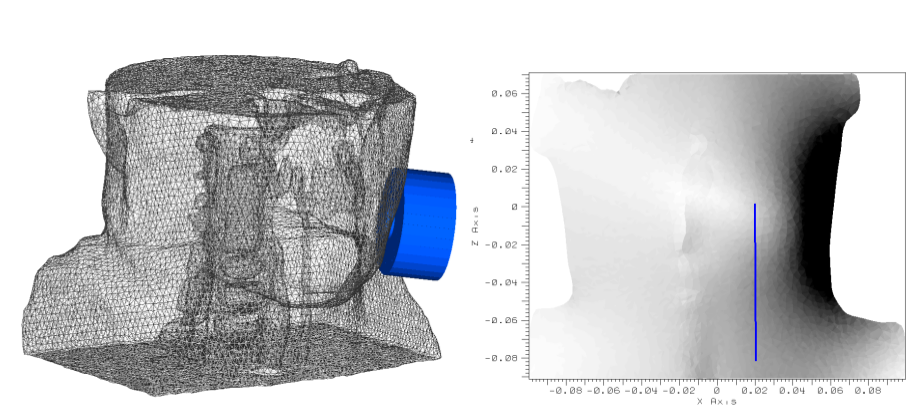
\includegraphics{pics/ecjext-mesh.png}

    Celem przykładu jest optymalne zaprojektowanie magnetycznego stymulatora
nerwu błędnego. Nerw błędny jest częścią autonomicznego układu
nerwowego. Nerw może być stymulowany elektrodami umieszczonymi
chirurgicznie w okolicach szyi, co pozwala zapobiegać napadom
padaczkowym i pomaga w walce z depresją.

Stymulacja magnetyczna pozwala uniknąć nacinania skóry i jest znacznie
bardziej bezbolesną metodą niż stymulacja elektryczna.

Równanie różniczkowe, rozwiązywane na modelu numerycznym ciała
człowieka, zdyskretyzowanym w postaci siatki czworościennej o 632808
krawędziach i 114405 węzłach.

    Parametry cewki 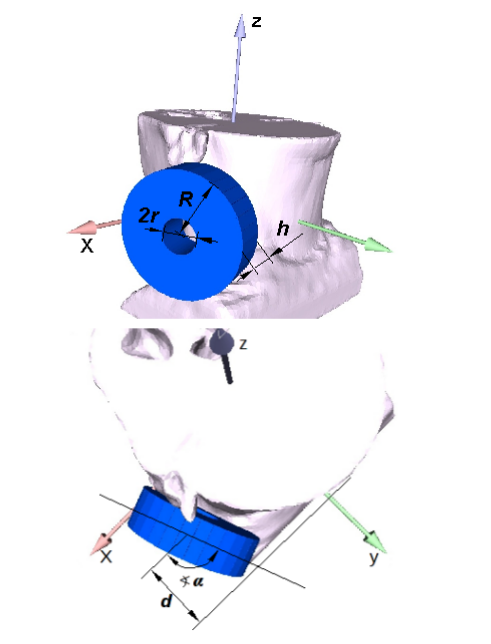
\includegraphics{pics/ecjext-param.png}

    Parametry cewki: promień zewnętrzny, wewnętrzny, odległość od
powierzchni skóry, kąt obrotu.

    Cewka o optymalnych parametrach i rozłożenie pola elektrycznego
indukowanego na powierzchni skóry. 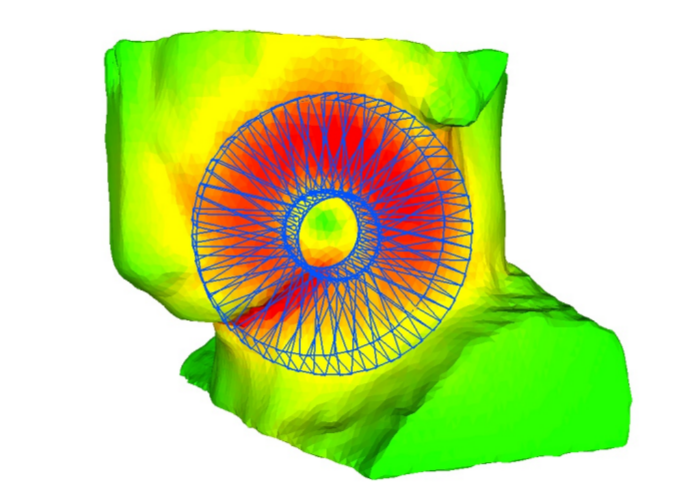
\includegraphics{pics/ecjext-opt.png}

    Ustawienia systemu równoległego 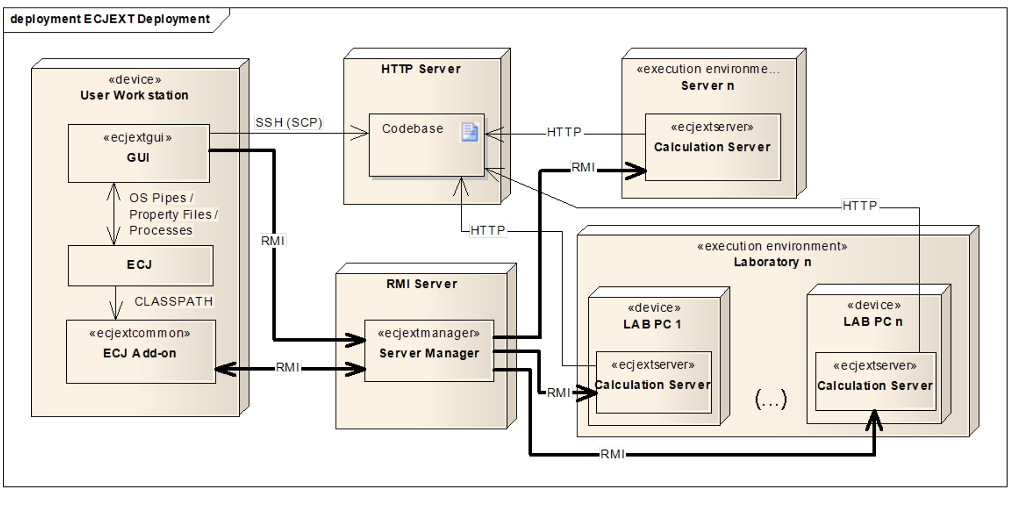
\includegraphics{pics/ecjext-depl.png}

    Przyspieszenie - praktycznie proporcjonalne do ilości użytych maszyn
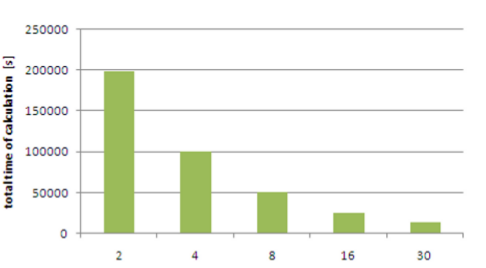
\includegraphics{pics/ecjext-speedup.png}

    Eksperymenty były przeprowadzone w uczelnianym laboratorium wyposażonym
w 30 komputerów (Core2Duo 2.4GHz + 2 GB RAM, system operacyjny Red Hat
Linux). Dla 30 komputerów całkowity czas rozwiązywania problemu wynosił
229 minut, dla dwóch maszyn - więcej niż 55 godzin.

    \subsubsection{Algorytmy genetyczne przy projektowaniu żywych
organizmów}

Ostatnio w wiadomościach na tvn mówiono o projektowaniu dzieci. Proces
miał polegać na sprawdzeniu genomu rodziców, generowaniu na ich
podstawie kilkunastu tysięcy cyfrowych płodów, na których możliwe było
sprawdzenie cech dzieci przed poczęciem.

    \section{Projektowanie algorytmów genetycznych}

\begin{enumerate}[1.]
\item
  Problem
\item
  Ocena rozwiązania
\item
  Sposób kodowania
\item
  Dobranie sposobu selekcji, krzyżowania, mutacji
\item
  Dobranie prawdopodobieństw krzyżowania i mutacji - raczej
  eksperymentalnie
\item
  Profit
\end{enumerate}

    \section{Hackathon!}

\begin{figure}[htbp]
\centering
\includegraphics{http://cdni.wired.co.uk/1240x826/g_j/Hackathon_1.jpg}
\caption{hackathon}
\end{figure}

    W marcu uczestniczyłem w fajnym wydarzeniu - Arday, gdzie słuchaliśmy
krótkich wykładów dotyczących platformy Arduino, a następnie mieliśmy
możliwość, w małych zespołach, przerabiać omawiany materiał w praktyce.
Chciałbym, wzorem tamtego spotkania, zrobić coś podobnego u nas.

Widzę to tak: paru z nas proponuje problemy, które następnie
rozwiązujemy w kilkuosobowych zespołach, z użyciem algorytmów
genetycznych. Na koniec prezentujemy efekty swojej pracy i cieszymy się,
że zrobiliśmy coś fajnego.

W razie gdyby brakowało pomysłów, mogę zaproponować kilka swoich.

    \subsubsection{Pomysły}

\section{??}

    Łatwe:

\begin{itemize}
\item
  Modyfikacja przykładowego programu - znajdowanie ekstremum funkcji
  zależnej od 2 zmiennych.
\item
  Dopasowanie funkcji
  $f^N, f \in [\exp, \sin, \cos, +, -, *, /, x_1 ... x_N]$ do zbioru
  danych
\item
  Znajdowanie tożsamości trygonometrycznych
\item
  Automatyczne testowanie wydajnościowe wybranego algorytmu sortowania
\end{itemize}

    Średnie

\begin{itemize}
\item
  Znajdowanie przybliżonych całek nieoznaczonych dla funkcji
  niecałkowalnych analitycznie np.
  $\exp(-x^2), \sin(x^2), \frac{sin(x)}{x},\frac{1}{ln(x)}, x^x$
\item
  Projektowanie obwodu elektrycznego o określonej charakterystyce
  (https://github.com/ahkab/ahkab/wiki/Example:-Python-API)
\end{itemize}

    Trudne

\begin{itemize}
\item
  Automatyczna gra w Tetrisa, Mario
\item
  Symulacja wybranego zjawiska fizycznego
\end{itemize}

    \begin{Verbatim}[commandchars=\\\{\}]
{\color{incolor}In [{\color{incolor}28}]:} \PY{k+kn}{from} \PY{n+nn}{IPython.core.display} \PY{k+kn}{import} \PY{n}{HTML}
         
         \PY{k}{def} \PY{n+nf}{css\PYZus{}styling}\PY{p}{(}\PY{p}{)}\PY{p}{:}
             \PY{n}{styles} \PY{o}{=} \PY{n+nb}{open}\PY{p}{(}\PY{l+s}{\PYZdq{}}\PY{l+s}{custom.css}\PY{l+s}{\PYZdq{}}\PY{p}{,} \PY{l+s}{\PYZdq{}}\PY{l+s}{r}\PY{l+s}{\PYZdq{}}\PY{p}{)}\PY{o}{.}\PY{n}{read}\PY{p}{(}\PY{p}{)}
             \PY{k}{return} \PY{n}{HTML}\PY{p}{(}\PY{n}{styles}\PY{p}{)}
         \PY{n}{css\PYZus{}styling}\PY{p}{(}\PY{p}{)}
\end{Verbatim}

            \begin{Verbatim}[commandchars=\\\{\}]
{\color{outcolor}Out[{\color{outcolor}28}]:} <IPython.core.display.HTML at 0x3aca490>
\end{Verbatim}
        

    % Add a bibliography block to the postdoc
    
    
    
    \end{document}
